\chapter{Theory of Dark Matter}
% add what does the different method excludes in the dark matter summary plot


\epigraph{\textit{One does not become enlightened by imaging figures of light, but by making the darkness conscious.}}{--Carl Jung}


\section{History}
    Dark matter is arguably one of the most solid evidence for beyond the standard model physics. In 1933, Fritz Zwicky first conceptualized the existence of a dunkle Materie ("dark matter") holding the galaxies to the cluster center and thus preventing them from flying apart ~\cite{Zwicky}. The proposition was later concurred by different findings by Horace W. Babcock ~\cite{Babcock} and Jan Oort ~\cite{oort}, among many others. The existence of such matter is also supported by evidence across different physics scales including the cosmic microwave background, and bullet cluster collision.

    Dark matter is known for interacting gravitationally and at most weakly (though recent evidence has shown weak scale interaction to be unlikely) with Standard Model particles . It does not interact electromagnetically or strongly. Its known properties does not match any known standard model particle. Very little is known about its composition and and interaction mechanism. However, as dark matter makes up about 85\% of the matter in the universe ~\cite{Hinshaw_2013}, five times more than the ordinary matter covered in previous chapter. Its discovery would lead to breakthrough in human understanding about the universe. Afterall, dark matter plays a major role in astro-object mechanics, galactic cluster formation and the evolution of the universe. Without a proper understanding of dark matter and its composition, human understanding of the universe will be incomplete.

    Experiments and observations over the years have contricted some dark matter properties, but much of the physics is still remains a mystery. It is generally accepted that dark matter is a particle. Various ways have been developed to study the mystery particle in telescope, earth based detector and colliders. In the LHC, it is believed that dark matter can be studied through direct production. If dark matter can be produced in a laboratory, it will make probing many of its other properties possible. 

    In this chapter, evidence for the existence of dark matter will first be reviews in 3.1, dark matter and the current properties that restrict its nature will be covered in 3.2; section 3.3 reviews possible dark matter candidates; an overivew of search method for dark matter is covered in 3.4,  highlights on the theoretical model used by the LHC that studied dark matter is discussed in 3.5. Lastly, LHC dark matter search signatures are included in 3.6.

\section{Evidence}

\subsection{Galactic Rotational Curve}
    The first proposition of dark matter in 1930s in the Coma cluster by Fritz Zwicky and others was later confirmed by further systemic galaxy rotational curve studies by Vera Rubin, Kent Ford ~\cite{Rubin} and Ken Freeman ~\cite{freeman}.  
    Following Zwicky's original argument, galactic clusters and galaxies can be treated as a stable system of discrete particles in astrophysical scale, and is therefore govern by the Virial theorem:
% Rubin and Ford studied galaxy M31 region and found that different region moves at a different speed than expected of the mass of the galaxy
%



    \[ \langle T \rangle = -\frac{1}{2} \sum_{k=1}^{N} \langle F_{k} \cdot r_{k} \rangle

    The Virial theorem shows that the there is a direct correlation between the kinetic energy and potential energy in a galactic system. Thus there is a correlation between the velocity of the rotating galactic cluster disk and the mass (through gravitational force) of the system. The correlation that allows for a stable system is as follow:
    
     \[ v(r) \varpropto \frac{M(r)}{\sqrt{r}} \], where r is the distance from the center of the system.

    Outside of the system, M(r) is a constant, the formula can be further simplified to:

     \[ v \varpropto \frac{1}{\sqrt{r}} \], 

    However, in observation, it was found that the velocity for many of these cluster is close to constant to r. It is proposed that there is a missing dark halo of dark matter that is not illuminous. Through these studies, it was found that ordinary luminous matter only could account for one-sixth of the matter in some galaxies.

\begin{figure}[!htb]
    \begin{center}
        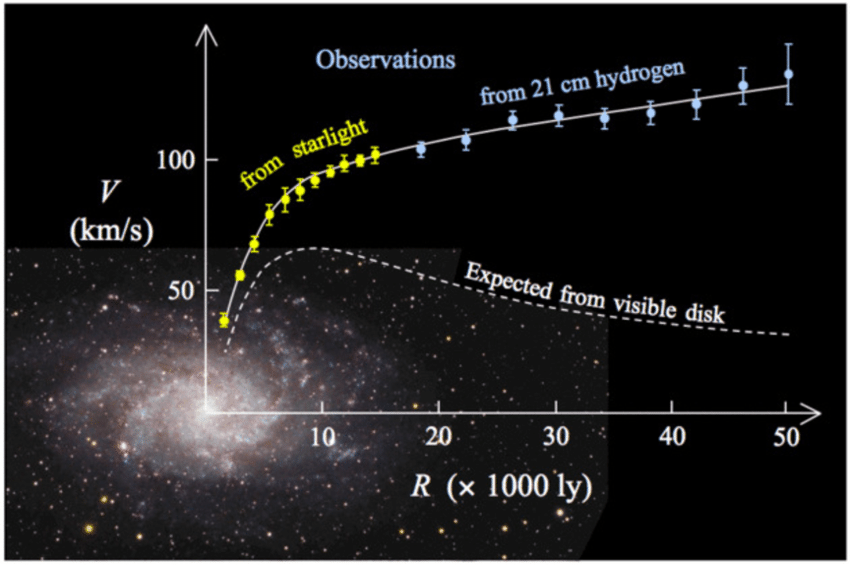
\includegraphics[width=0.75\textwidth]{figures/chapter_DM/M33-rotation-curve}
        \caption{
            Figure here shows the galactic rotational curve of M33, the expected rotational curve is shown in the dotted line. Experimental evidence observes behavior in the solid line.~\cite{M33}.
        }
        \label{fig:M33_figure}
    \end{center}
\end{figure}


\subsection{Gravitational Lensing}

    General relativity shows that massive objects would curve and modify the space-time curvature around them. Light ray travelling through the curved space-time around the massive object would therefore be bent. The effect mirrors that of angled lenses bending light rays due to a velocity differece of light ray across different media and is called gravitational lensing. There are different forms of lensing effect, roughly arranged by the strength of their effects. Strong lensing effect happens when bending of light result in either multiple images, a light ring or an arc, more typically observed around massive centers of galaxy clusters and galaxies; whereas weak lensing usually involves statistical analysis of many objects over a large region; micro-lensing is detected when there is an apparent change in the brightness of the source.

    Figure~\ref{fig:BulletCluster_figure} shows the bullet cluster collision of 1E 0657 -56. It is produced from the combination of gravitational lensing and x ray telescope imaging. The red part of the diagram denotes ordinary matter and the blue part reflects dark matter. In the cluster collision, ordinary matter bend light around them and became luminous from the collision, captured by x-ray imaging; the blue part shows a part of the clusters that did not interact and light up in the collision via gravitational lensing. This is a strong evidence for the existence of non-luminous matter in the clusters.

\begin{figure}[!htb]
    \begin{center}
        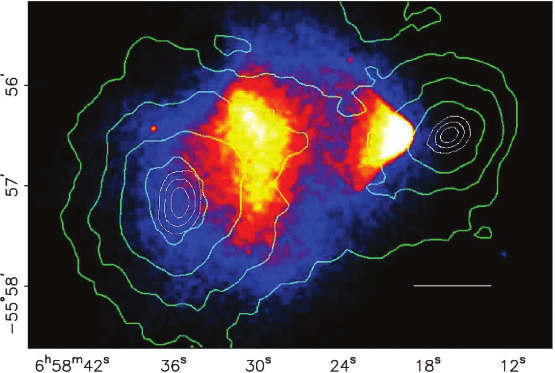
\includegraphics[width=0.75\textwidth]{figures/chapter_DM/BulletCluster}
        \caption{
			Bullet cluster (1E 0657-56) showing two colliding galaxy clusters, the part in red came from x-ray image by Chandra, highlighting normal matter distribution; the part in blue came from gravitational lensing. ~\cite{BulletCluster}.
        }
        \label{fig:BulletCluster_figure}
    \end{center}
\end{figure}


\subsection {Cosmic Microwave Background}

    In the beginning of the universe, ordinary matter and dark matter all exist in a hot plasma soup with frequent interaction between charged particles and photons through thomson scattering. There comes a very important period in the universe called the recombination period, where the expansion of the universe has cool the plasma soup enough that charged particles began to form neutral atoms. Photons stopped scattering on the charged particles and went on unhindered. Due to red
shifting effect, they form a microwave background of the universe that can still be observed today. This is the Comic Microwave Background. 
This original background is nearly a black body and is therefore very uniform, but there exists small temperature variations. The variation can be decomposed into an angular power spectrum, as shown in Figure~\ref{fig:CMB_figure}
Due to the different interaction between dark matter and ordinary matter with photon and each other, simulation shows that different dark matter and ordinary matter make-up of the universe would result in different angular spectroscopy shape. 
Study from Planck on cosmic microwave background Figure~refgives a clear composition and percentage abundance of dark matter. Dark matter is not only an essential part of the universe, its composition is approximately 5 times as large as ordinary matter. Giving evidence that dark matter makes up the majority of the universe. 
%\figure planck 

\begin{figure}[!htb]
    \begin{center}
        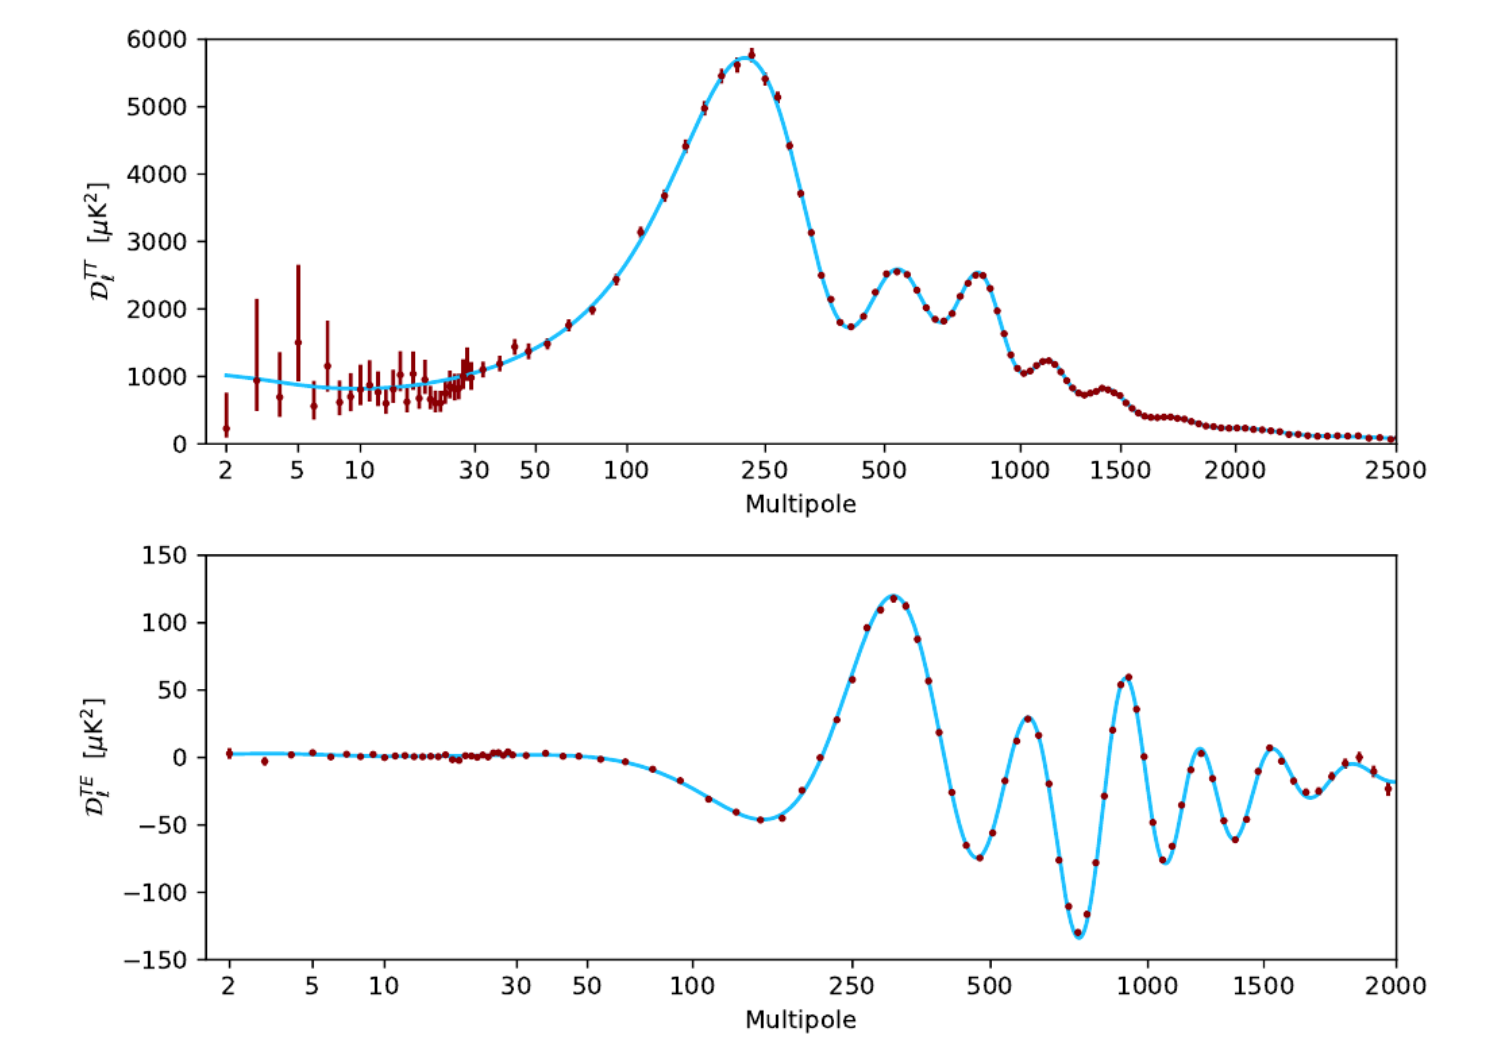
\includegraphics[width=0.75\textwidth]{figures/chapter_DM/CMB-angular-power-spectrum}
        \caption{
			The Cosmic Microwave Background power spectrum measured by Planck.~\cite{CMB}.
        }
        \label{fig:CMB_figure}
    \end{center}
\end{figure}




\section{Properties}
While dark matter itself has never been directly observed, many studies in the cosmological, astrophysical and particle scale has constrained much of its properties. In this section and the remaining thesis, the following properties of dark matter will be assumed along with its justifications.

\subsection{Dark}
Dark matter got its name from its little to no interaction with light compared to ordinary matter in cosmological observation. Collision of the bullet cluster has also greatly constrained its interaction with itself.  
It is taken that it will not interact with collider detector and its interaction with ordinary matter would be rare in the energy scale of the LHC. 

\subsection{Long Life Time}
In the particle model of dark matter, many requires a $Z_{2}$ symmetry (such as the R parity of supersymmetry). This prevent dark matter particles from decaying into lighter Standard Model objects. In most LHC analyses, it will be treated as a single object that does not decay further into other detectable SM particles. ~\cite{boveia2018dark}

\subsection{Cold}
In cosmology, hot/cold refers to the relativistic mass of an object and thus their relativistic velocity in cosmological scale evolution. Different assumption of the relativistic mass of dark matter has great impact on the cosmological evolution/ galactic formation in cosmology.
As a hot relativistc model of dark matter will lead to cotradiction in galactic formation and universe evolution calcuation. Dark matter is taken to be non-relativistic by most physicists. 

\subsection{Single Particle}
While there are more and more composite dark matter models being proposed these days, dark matter is still taken to be a single kind in most effective model/simplified model building for experimental searches. 

\section{Candidates}

There exist a wide range of candidates for what dark matter could be. In here, I outline a few possible candidate of dark matter. , other than candidates include sterile neutrinos, axion dark matter weakly interacting  

\subsection{Sterile Neutrino}
Standard model does not predict that neutrino has a mass, however, that contradicting with experimental finding and is therefore a problem of the standard model. By replacing right-handed neutrinos in the standard model with gauge singlet fermions that has no interaction other than mixing with normal neutrinos, sterile neutrino is formed by theoretical models. Tuning parameters such its interaction rate with normal neutrino, mass and mixing angle, sterile neutrino can be a possible candidate for dark matter, as it can lead to a right
density of dark matter with stability consistent with the scale of the universe. ~\cite{dodelson1994sterile} They are searched for in radiator experiments such as the Daya Bay \cite{an2014search, wong2017search} and in scintillator experiments like DANSS. ~\cite{alekseev2018search}

% Mass and range  mass keV scale, currently sterile neutrino mass is unknown and therefore can be either hot or cold

%Daya Bay Collaboration, F. P. An et al., “Search for a Light Sterile Neutrino at Daya Bay,” Phys. Rev. Lett. 113 (2014) 141802, arXiv:1407.7259 [hep-ex].
%1310.8642
\subsection{Axion Dark Matter}
Another exisitng problem in the standard model is the strong CP problem. The strong CP problem points to the unnaturalness of CP symmetry observed in neutrons charge distribution measurement. This gives an exceptionally small value to the term that govern strong CP violation in the Standard Model, which is unnatural. The problem can be solved by introducing an additional axion particle and its associated fields to the standard model. ~\cite{peccei1977cp} With the proposition of such field, the CP violation term in strong interaction will be cancelled out naturally, thereby giving an explanation to the unnaturalness to the experimental value. 
The axion proposed is a dark matter candidate, as its calculated life time is much greater than the age of the universe and it shares many properties with the known profile of dark matter. Recent experimental finding from the XENON1T and shows anomalies that could be signs of axions. ~\cite{aprile2020excess}
%ADMX mass mu eV
%https://arxiv.org/pdf/2105.01406.pdf

%Xenon Collaboration, E. Aprile et al,. "Excess Electronic Recoil Events in XENON1T", Phys. Rev. D 102, 072004 (2020), arXiv: 2006.09721


% Non-particle candidates
%\subsection{Modified Newtonian Gravity}
%\subsection{MACHOs}

\subsection{Weakly Interacting Massive Particle (WIMP)}
A very attractive candidate for dark matter is called the weakly interacting massive particle(WIMP). It appears naturally with many beyond-the-standard-physics model that aim to solve other physics problems, including theories of supersymmetry with R-parity and some extra dimensional theory. 
In the study of dark matter in cosmology, it is frequently assumed to be a thermal relic. Thermal relic dark matter is in thermal equilibrium with ordinary matter in the early universe. In thermal equilibrium with ordinary matter, it gets produced and annihilated at the same rate. There comes a point in the universe called freezing out, where the expansion of the universe cools the particle bath and produce temperature lower than possible to produce enough energy statistically for dark matter to
be produced given certain dark matter mass. Dark matter production from ordinary matter ceased. As the universe further expanse, it becomes more difficult for dark matter to find each other to be annihilated to form ordinary matter. Dark matter abundance is locked at this point and remained unchange until today. 
Using this model and the current measured abundance of dark matter in our current universe, the self annihilation cross section of dark matter is $ \langle \sigma \cdot v \rangle \simequal 3 \cdot 10^{26}cm^{3} s^{-1}$. This annihilation cross section scale matches many prediction made in supersymmetry theories. Many beyond-the-standard-model theories, such as SUSY, the Universal Extra Dimension Model, and the little Higgs all predict a particle with known dark matter properties and self interaction rate of the same scale. This is known as the WIMP miracle. ~\cite{Dev_2014}

%\Figure WIMP miracle


\begin{figure}[!htb]
    \begin{center}
        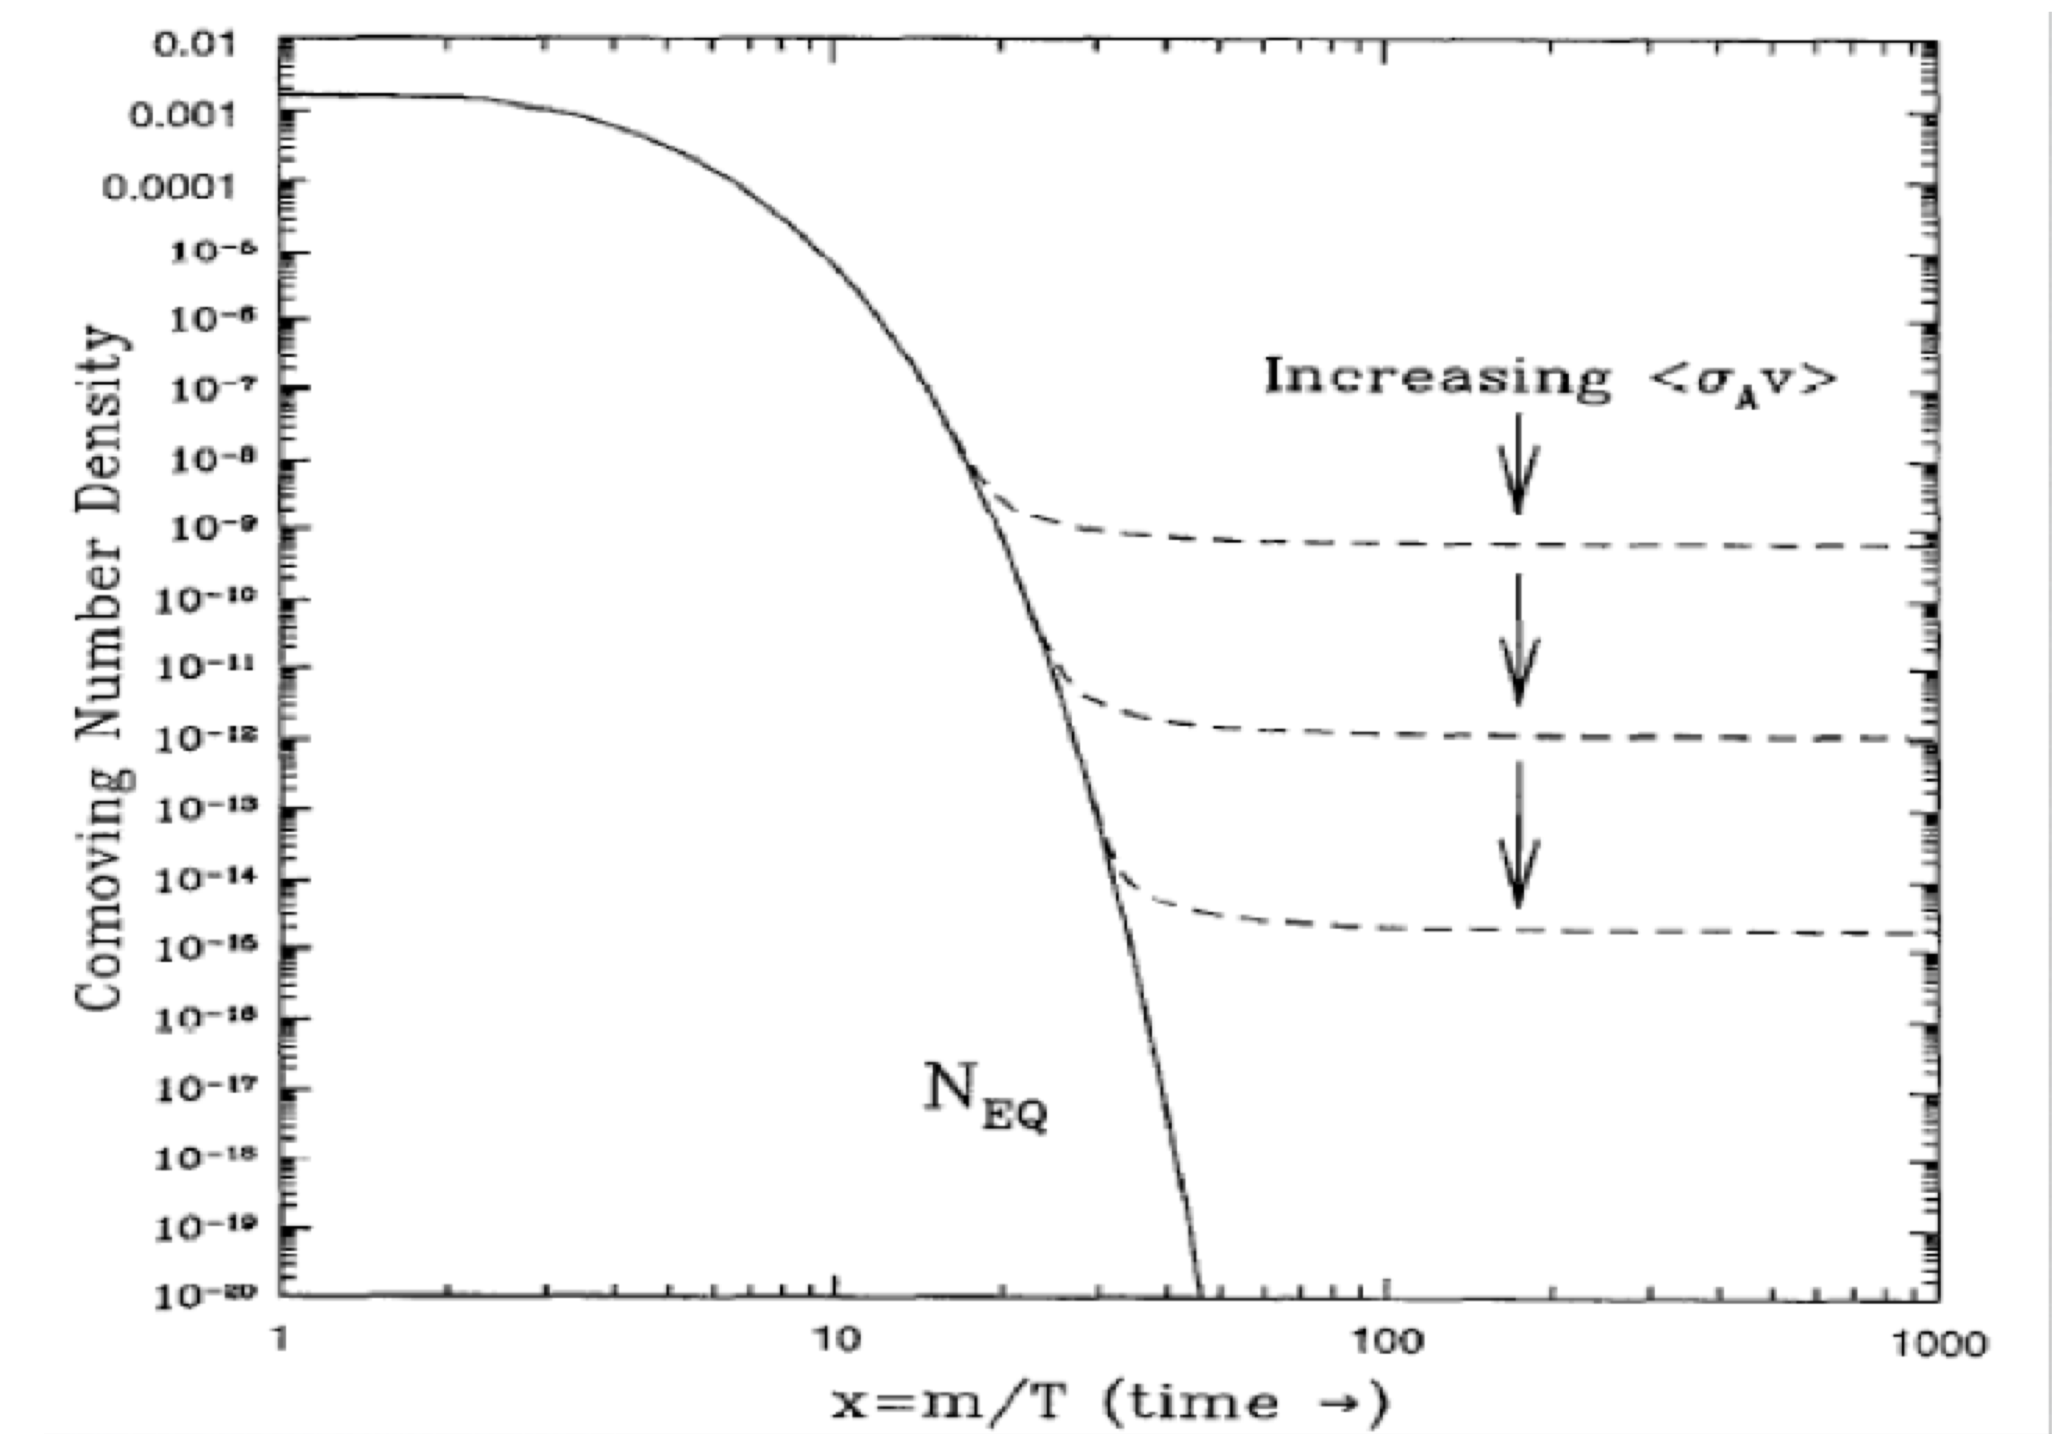
\includegraphics[width=0.75\textwidth]{figures/chapter_DM/WIMP}
        \caption{
		Solid line here shows the change in the densitiy of dark matter in an expanding unverse. In the early universe, the solid line is horizontal, indicating the time when dark matter production and annihilation is equal. The line gradually fall with increase of time when production rate began to decrease with the universe expansion. Later as the universe further expands, the annihilation stops as well and dark matter gets freezes out to different density level with different assumed self interaction annihilation rates.~\cite{WIMP}.
        }
        \label{fig:WIMP_figure}
    \end{center}
\end{figure}


 

%P.S. BHUPAL DEV, ANUPAM MAZUMDAR, & SALEH QUTUB, FRONT.IN PHYS. 2 (2014) 26
%https://indico.cern.ch/event/473000/contributions/1993414/attachments/1209863/1764345/tait-Aspen.pdf

%https://www.particlebites.com/?p=7004
%https://www.forbes.com/sites/startswithabang/2019/02/22/the-wimp-miracle-is-dead-as-dark-matter-experiments-come-up-empty-again/?sh=5ebc59f46dbc

\section{Experimental Search Overview}
Traditionally the search for dark matter is split into different experimental categories sorted by the different detection methods from different dark matter/normal matter interactions. 

\begin{figure}[!htb]
    \begin{center}
        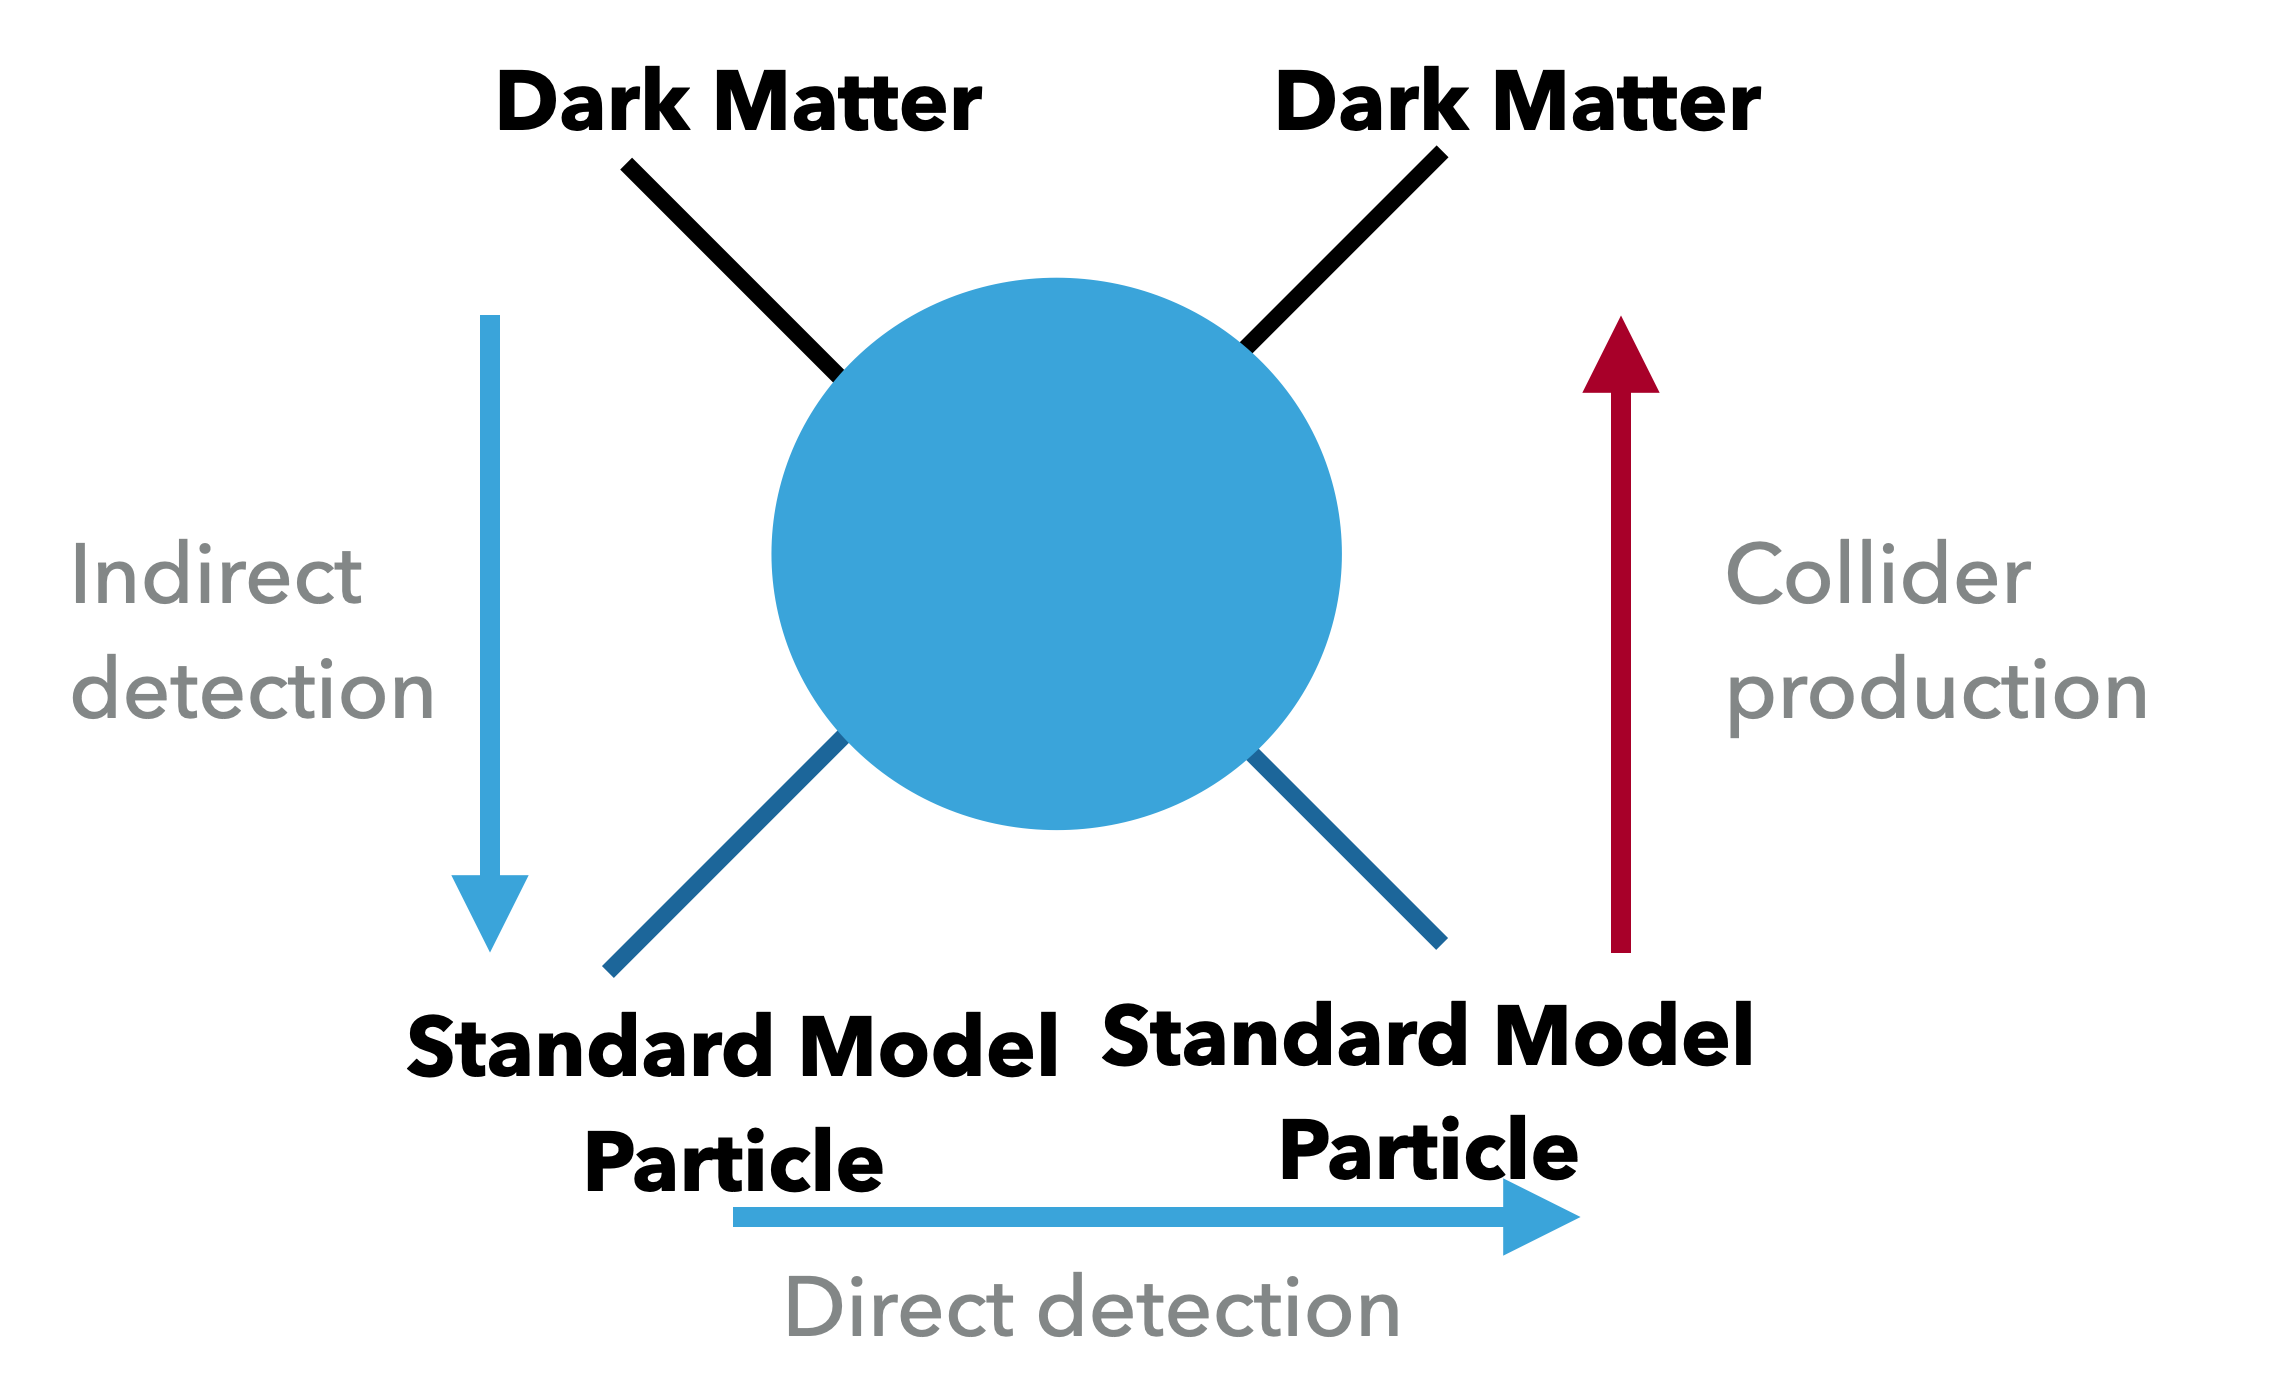
\includegraphics[width=0.75\textwidth]{figures/chapter_DM/Interaction}
        \caption{
			Schematic cartoon showing the different dark matter detection methods facilitated by different interactions thus signatures. 
        }
        \label{fig:interaction}
    \end{center}
\end{figure}

\subsection{Direct Detection}
Dark matter is believed to travel through the universe and passes through the eath. Assuming weak interaction between dark matter and Standard Model nucleons, dark matter can be detected directly with different target objects. 

\[ R \propto N \rho \chi \langle \sigma_{\chi } N \rangle \]

There are different experiments that uses different material and targets different dark matter masses.
Notable experiments include LZ ~\cite{mckinsey ~\cite{mckinsey2016lz},   Xenon1T ~\cite{aprile2020excess}, SuperCDMS ~\cite{Agnese_2016}, CRESST ~\cite{Angloher_2014} and DAMA ~\cite{Bernabei_2008}. 

As more and more experiments has excluded more and more of the model phasespace, many of the experiments now faces the challenge of the neutrino floor in low mass dark matter search, which is where neutrino background began to dominate signal region. 


%[29] DAMA Collaboration, R. Bernabei et al., “The DAMA/LIBRA apparatus,” Nucl. Instrum. Meth. A592 (2008) 297–315, arXiv:0804.2738 [astro-ph].
%[30] SuperCDMS Collaboration, R. Agnese et al., “New Results from the Search for Low-Mass Weakly Interacting Massive Particles with the CDMS Low Ionization Threshold Experiment,” Phys. Rev. Lett. 116 no. 7, (2016) 071301, arXiv:1509.02448 [astro-ph.CO].
%[31] CRESST-II Collaboration, G. Angloher et al., “Results on low mass WIMPs using an upgraded CRESST-II detector,” Eur. Phys. J. C74 no. 12, (2014) 3184, arXiv:1407.3146 [astro-ph.CO].
%[32] LUX Collaboration, D. S. Akerib et al., “The Large Underground Xenon (LUX) Experiment,” Nucl. Instrum. Meth. A704 (2013) 111–126, arXiv:1211.3788 [physics.ins-det].
%[33] XENON100 Collaboration, E. Aprile et al., “The XENON100 Dark Matter Experiment,” Astropart. Phys. 35 (2012) 573–590, arXiv:1107.2155 [astro-ph.IM].
#TODO
% L. Baudis, “Direct dark matter detection: the next decade,” Phys. Dark Univ. 1 (2012) 94–108, arXiv:1211.7222 [astro-ph.IM].

\subsection{Indirect Detection}
Indirect detection looks for annihilation Standard Model product of dark matter. It looks for interaction in places where matter is dense enough to interact, usually in center of galaxies and stars. Experiments include FermiLAT ~\cite{albert2017searching} and H.E.S.S. ~\cite{aharonian2006hess}


\subsection{Collider Production} 
    In the Large Hadron Collider, dark matter can be studied by being directly produced from Standard Model particles. Here, a few signatures are discussed. 

\section{Theoretical Models in LHC Searches}

While there exist a wide range of speculation on the identity of dark matter, the use of LHC as a dark matter searching tool constrains a unique set of dark matter candidate accessible phenomenologically. 
Focusing phenomenologically observable and interpretability for a wide range of theoretical models, different modelling approaches are used to develop benchmark models searching for dark matter in the LHC.
Sorting by an ascending degree of completeness, the literature will review different approaches and models of dark matter used in the LHC.


\begin{figure}[!htb]
    \begin{center}
        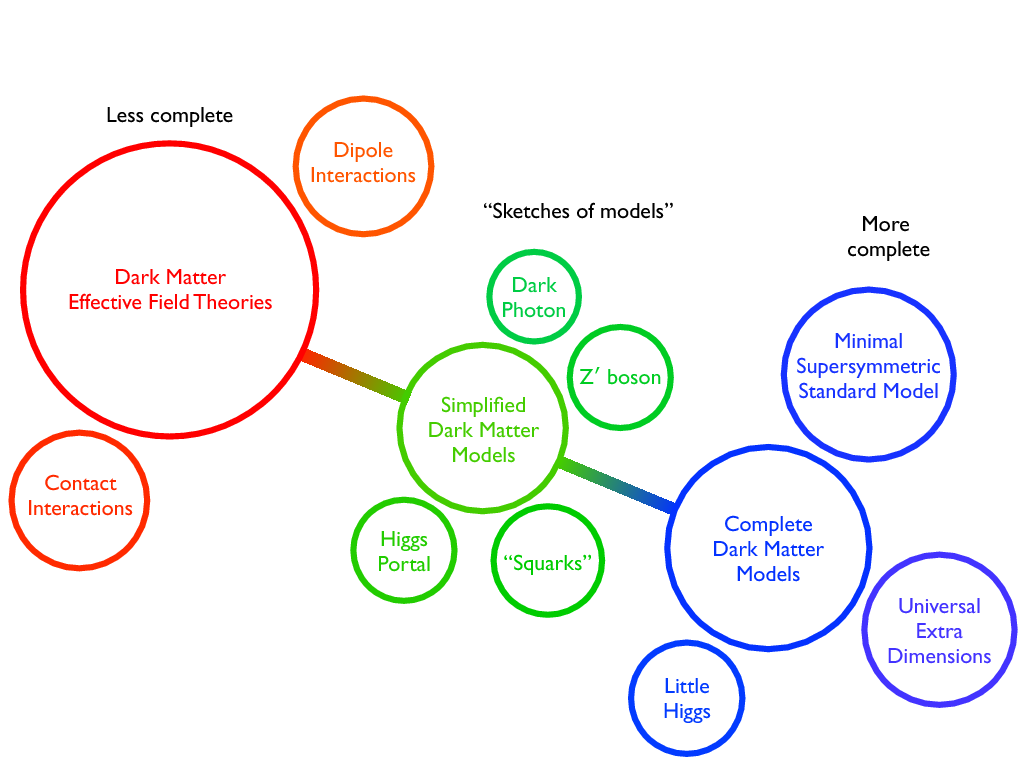
\includegraphics[width=0.75\textwidth]{figures/chapter_DM/Model}
        \caption{
			Colored Scheme showing dark matter modelling approach from more simplistic (left) to more complete models (right).  ~\cite{Abdallah:2024101}.
        }
        \label{fig:Model_figure}
    \end{center}
\end{figure}



\subsection{Simple Portal Models}
The simplest kind of models are simple extensions to the standard model. In these models, dark matter is mediated either through the Higgs or the Z Boson. As the Z portal models are contrained by LEP and DD experiments, dark matter that are mediated through a heavier version of Z boson ( the Z') and additional scalar is also searched for. 

\subsection{Effective Field Theory}
The effective field theory appraoch condense a wide range of complete models to simplified versions by focusing on what is experimentally accessible. High mass mediator particles in complete theories as a contact operator. High energy correction and details are integrated out for "effectiveness". All kinematically accessible observables are described by a Lorentz structure and a rate parameter. 
This approach allow for the easily measured experiment values and a framework for a wide range of complete models to be probe with few experimental model search. However, the model has a singularity and is not valid for when the interaction momentum transfer is close to that of the mediator mass. A truncation method is used to bound the events simulated Monte Carlo events below this limit.  

Giorgio Busoni, Andrea De Simone, Johanna Gramling, Enrico Morgante, and Antonio Riotto, On the validity of the e􏶺ective 􏶻eld theory for dark matter searches at the LHC, part II: complete analysis for the s-channel, JCAP, 1406:060, 2014.

\subsection{Simplified Model}
The problem in effective field theory can be resolved with the simplified Model appraoch. The contact interaction in EFT is turned into mediator particle s-channel/t-channel exchanges in simplified model. With the price of an increased number of parameters, simplified models can provide the full mechanics of a particle interaction and usually come with more details. 
Simplified models of dark matter in the LHC do not break the global and gauge symmetries of Standard Model, the Lagrangian terms are Lorentz invariant and predicts at least a dark matter candidate that fullfills the properties described in the previous section. 
Some simplified dark matter model used in the LHC include the Two-Higgs Doublet Model (2HDM), where Higgs or a non-standard model exotic higgs could serve as a mediator to dark matter; other examples include dark photon or a kinetically mixed Z' dark matter model. 
Other than these, simplified model in supersymmetry such as the Phenomenological Minimal Supersymmetric Standard Model (pMSSM) which reduces the over 100 parameters of complete model of Minimal Supersymmetric Standard Model to 19 parameters, predicts candidate dark matter like particles, predicts neutralino as a natural dark matter candidate. 
In addition, other gauge or gravity mediated SUSY theory predicts gravitino as a dark matter candidate. 
% pMSSM Assumes no sources of CP violation beyond the Standard Model and no flavor-changing neutral currents, and retains uni- versal couplings and masses for first- and second-generation superpartners. %CatDog Antonio DM summary paper.  

\subsection{Less-simplified models}
\subsection{Long-Lived Particle Models}

A detail list of models used by the LHC by both the CMS and ATLAS can be found in this reference https://arxiv.org/pdf/1507.00966.pdf

\section{Experimental Signature in the LHC}

\subsection{Mono-X signature}
    This describes the type of dark matter search where an invisible dark matter is produced directly in the LHC and is "observed" in the detector as missing transverse momentum.
    Dark matter is known to interact only very weakly with normal matter, and thus is assumed to not leave a trace in the LHC detector. When events are produced through proton-proton collision along the z-axis in the LHC, the momentum of all objects along the transverse plane to the z-axis is always zero. Therefore, when an event has missing transverse momentum recoiling against another visible object, the signature would possibily be dark matter.
This class of analysis is named by the standard model object that dark matter recoil against. Mono-jet, mono-Higgs, mono-Z are a few analyses done this way. 

\subsection{Di-object Signature}
    Dark matter can also be searched for without the production of the dark matter particle. The simplified models that predicts dark matter in the mono-X analyses predicts effective mediator particle between standard model particle with dark matter. These effective mediator particles can be directly searched for through via decay back into standard model object. As the process is distinct from any known Standard Model particle processes, an excess of events beyond standard model prediction for
    such a mediator process could be evidence for dark matter in the LHC. 
These di-object search include dijet, dilepton, diphoton searches. 
In recent years, new techniques such as the trigger-level-analysis and channels that has an additional initial state radiation objects are being pioneered. These result in a search phasespace much greater than the traditional program and greatly extended the of the richness of the LHC serach program.

\subsection{Long-Lived Particle Signature}


% compare the strenght of the different method in probing the dark matter models discussed. 



%%%%%%%%%%%%%%%%%%%%%%%%%%%%%%%%%%%%%%%%%%%
%%%%%%%%%%%%%%%%%%%%%%%%%%%%%%%%%%%%%%%%%%%
%% sub section describing SM particle content and lagrangian
%%%%%%%%%%%%%%%%%%%%%%%%%%%%%%%%%%%%%%%%%%%
%%%%%%%%%%%%%%%%%%%%%%%%%%%%%%%%%%%%%%%%%%%
%\section{Particles and Forces}
\label{sec:sm_description}

There are four known fundamental forces at work in the universe: electromagnetism,
the weak interaction, the strong interaction, and gravity.
Our understanding of the existence of each of these forces
has essentially been arrived at empirically, with physicists following experimental
clues, and their basic behaviors deduced after long trials of effort.
The SM encompasses all of these forces except for gravity, which currently
is only described by the classical (i.e. not quantum) theory of geometrodynamics, or general
relativity.
The gravitational interaction is incredibly weak in comparison to the others, however, and
is not relevant to the types of particle interactions that we are currently
sensitive to in particle physics experiments.
Electromagnetism is by far the most familiar, as it is the force
most commonly experienced and is what is at work in our everyday life (reaction forces between
objects on tables and chairs, friction, wall-plugs, batteries, DNA structure, etc...) and is typically what
students are first presented with in their physics studies.
The weak force is responsible for things like radioactive decay,
which makes possible the process of nuclear $\beta$-decay and the nuclear
fission process that fuels the sun, for example. The strong force is what binds protons
and neutrons together, and thus is responsible for holding together most of the (ordinary) matter
in the universe.\footnote{`Ordinary' to distinguish from dark matter, for example.}

The forces mediate the interactions between the matter particles, which we use to deduce
their presence. The SM predicts fundamental, point-like particles that appear in two
general classes depending on whether they have integral spin ($\mathcal{S} \in [0,1,2,...)$) or half-integral
spin ($\mathcal{S} \in [1/2, 3/2, ...)$); the former are referred to as \textit{bosons} and the
latter as \textit{fermions}.
In the SM, the particles that are responsible for making up matter are all spin-$1/2$ fermions
and are either \textit{leptons} or \textit{quarks}; within each class
there are three generations (or families) that are essentially copies of the first.
The forces in the SM are interpreted as being mediated by spin-$1$ bosons, referred to as the 
\textit{gauge bosons}.
The leptons and quarks all experience the weak force, but only the quarks experience
the strong interaction. All electrically charged particles interact with the electromagnetic
interaction.

The particles of the SM are described as quantum fields whose dynamics are
described by the SM Lagrangian from which the equations of motions can be derived.
The particles, and by extension the SM Lagrangian that describes them, are found to be invariant under transformations of spacetime 
(space translations, rotations, Lorentz boosts) and three internal transformations described by unitary transformations: $\mathcal{P} \times$\SUthree$_C \times $ \SUtwo$_L \times$ \Uone$_{Y}$.
This is illustrated in Figure \ref{fig:sm_forces}. The strong force is described by a
local \SUthree~symmetry that acts only on the particles that have \textit{color charge}.
The term ``color'' arises from the fact that the color charge is found to exist
in three varieties which have been labelled as red (r), blue (b), or green (g), and due
to the fact that ``colorless'' states are formed when all three are combined (r+g+b), just
like with visible light that humans are familiar with, or when states are formed of color-anti-color
pairs (r+$\bar{\text{r}}$). For this reason, the QFT describing the strong force is called
Quantum \textit{Chromo}dynamics (QCD), and is mediated by eight \textit{gluons} (\fieldG).
The particles subject to the weak force are invariant under weak-isospin \SUtwo~transformations,
mediated by the three  \fieldW~bosons (\fieldWone, \fieldWtwo, \fieldWthree).
The \Uone~transformations, mediated by the \fieldB~boson, preserve weak-hypercharge, $Y$.
The \SUtwo~symmetry is respected only by the left-handed chiral
particles (leptons or quarks), with the right-handed chiral particles not participating.
There is additionally a single scalar (i.e. spin-0) field, the Higgs field, that is an \SUtwo~doublet, about which more will be described shortly.
The particle content thus described is presented in detail in Table \ref{tab:sm_content}.
The \SUtwo~left-handed chiral fields appear as doublets and are grouped in
and `up-down' pair (e.g. (\fieldUl, \fieldDl) or (\fieldEl, \fieldNuEl)) whereas the right-handed chiral fields,
living in the singlet representation of \SUtwo, do not (e.g. \fieldUr)). Note
that the SM does not allow for right-handed neutrinos (a term like \fieldNuR~does not appear).

\begin{figure}[!htb]
	\begin{center}
		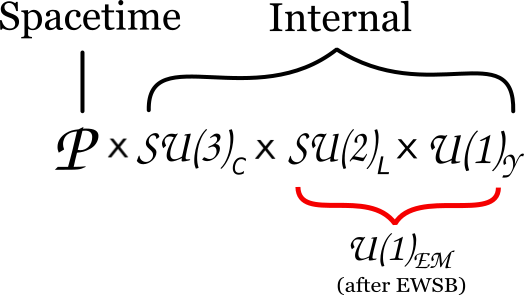
\includegraphics[width=0.5\textwidth]{figures/chapter1/sm_forces}
		\caption{
			The spacetime and internal gauge structure of the SM.
			$\mathcal{P}$ refers to the Poincar{\'e} symmetry group.
			\SUthree$_c$ refers to the \SUthree~symmetry
			of the color sector of QCD and \SUtwo$_{L}\times$\Uone$_{Y}$ refers to the left-handed chiral
			symmetry of the electroweak interaction. After spontaneous symmetry
			breaking due to the Higgs mechanism, the \SUtwo$_L \times$ \Uone$_Y$ symmetry
			reduces to the \Uone$_{EM}$ symmetry of electromagnetism. 
		}
		\label{fig:sm_forces}
	\end{center}
\end{figure}
\FloatBarrier

The SM Lagrangian is shown in Equation \ref{eq:sm_lagrangian} and describes the complete
content of the SM: encompassing all interactions between the known particles and the
symmetries that they obey.

\begin{align}
	\mathcal{L}_{\text{SM}} = -\frac{1}{4} \sum\limits_{\text{gauge}} \mathit{F}_{\mu \nu}^i \mathit{F}^{i\,\mu\nu}
	- \sum\limits_{f} \bar{f}\gamma^{\mu} \mathit{D}_{\mu} f 
	+  (\mathit{D}_{\mu} \phi)^{\dagger} (\mathit{D}^{\mu} \phi) - \mu^2 \phi^{\dagger}\phi - \lambda(\phi^{\dagger}\phi)^2
	\label{eq:sm_lagrangian}
\end{align}
\noindent
The first term of Equation~\ref{eq:sm_lagrangian} is a sum over the three internal gauge groups,  and $\mathit{F}^a_{\mu \nu} = \partial_{\mu} \mathit{A}_{\nu}^a - \partial_{\nu} \mathit{A}_{\mu}^a + g f^{abc} \mathit{A}_{\mu}^{b}\mathit{A}_{\nu}^{c}$, where $\mathit{A}_{\mu}$ is one of the
three gauge fields, $g$ is the associated gauge coupling parameter, and a sum over $i$ is implied. The $f^{abc}$ are the so-called
\textit{structure constants} of the gauge group. For Abelian groups like \Uone, $f^{abc}$ = 0.
For non-Abelian gauge groups like \SUtwo~and \SUthree, $f^{abc} \ne 0$. For example, for
\SUtwo~the structure constants are nothing more than the Levi-Civita totally anti-symmetric tensor, 
$\varepsilon_{ijk}$, giving for the weak gauge force:
\begin{equation}
	\mathbfcal{W}_{\mu \nu} = \partial_{\mu} \mathbfcal{W}_{\nu} - \partial_{\nu} \mathbfcal{W}_{\mu} - g_2 \mathbfcal{W}_{\mu} \times \mathbfcal{W}_{\nu}
\end{equation}
where $\mathbfcal{W}_{\mu}$ is the vector of the three weak gauge fields (\fieldWone, \fieldWtwo, and \fieldWthree) and $g_2$ is their associated gauge coupling. The non-zero $f^{abc}$ of non-Abelian gauge groups means that the gauge bosons of
the weak and strong interactions can interact with themselves due to terms appearing in Equation
\ref{eq:sm_lagrangian} that contain only the gauge bosons.

The second term of Equation~\ref{eq:sm_lagrangian} describes the lepton and quark kinetic energies and their interactions with the gauge fields.
The $f$ refer to the fermion fields (quarks and leptons) and the corresponding sum is over all
species of fermion. $\mathit{D}_{\mu}$ is the gauge covariant derivative, and for the SM is
given by:

\begin{equation}
	\mathit{D}_{\mu} = \partial_{\mu} - i g_1 \frac{Y}{2} \mathcal{B}_{\mu} - i g_2 \frac{\tau^i}{2} \mathcal{W}_{\mu}^i - i g_3 \frac{\lambda^a}{2} G_{\mu}^a
	\label{eq:gauge_derivative}
\end{equation}
where $g_1$, $g_2$, and $g_3$ are the gauge coupling constants for \Uone$_{Y}$, \SUtwo$_{L}$, and \SUthree$_{C}$, respectively, that give the overall strength of the associated coupling.
Summation over repeated indices is implied and the $\tau^i$ ($\lambda^a$) are the three (eight)
generators of the \SUtwo~(\SUthree)~gauge group, with $i \in [1,2,3]$ ($a \in [1,..,8]$), and
are typically represented by the Pauli (Gell-Mann) matrices. Note that the form of Equation~\ref{eq:gauge_derivative} is strictly mandated by the requirement that the theory
be \textit{gauge invariant}, i.e. that transformations of the fields under the internal symmetries
of Figure \ref{fig:sm_forces} leave the action of $\mathcal{L}_{\text{SM}}$ unchanged.
%This is described in detail in {\color{red}{Appendix XXX}}.

The last three terms in Equation \ref{eq:sm_lagrangian} are all terms including the Higgs field, $\phi$,
and will be discussed in detail in Section~\ref{sec:higgs_description}.

Inspection of Equation~\ref{eq:sm_lagrangian} will reveal two things. The first thing that one
may notice is that it does not appear to describe electromagnetism as it does not have a
term representing the photon, the familiar mediator of the electromagnetic interaction.
The second, and perhaps more immediately obvious, thing is that no mass terms
appear in $\mathcal{L}_{\text{SM}}$: all fields appear to have zero mass! Both of these
facts are counter to our everyday experience: we know electromagnetism is real and that matter,
at the very least, is massive. In the next few sections we will see how these apparent
issues are resolved.


\begin{table}[!htb]
    \caption{
        The particle content of the SM and their transformation
        properties under the SM gauge groups, prior to electroweak symmetry breaking.
        The representations of each of the gauge groups are shown in the three-right
        columns. The \Uone symmetry of weak-hypercharge transformations is one-dimensional
        and the column gives the weak-hypercharge $\mathcal{Y}$ associated with each
        field. For \SUthree and \SUtwo, $\mathbf{1}$ refers to the field belonging to
        the associated singlet representation, $\mathbf{2}$ to the doublet representation,
        $\mathbf{3}$ to the triplet representation, and $\mathbf{8}$ to the octet representation.
    }
    \begin{center}
        \begin{tabularx}{0.96\textwidth}{m{1em} c c c c c c c }
        \toprule
        \hline
        & Field Label & Content & Spin & \Uone~($\mathcal{=Y}$) & \SUtwo & \SUthree \\
        \hline
        \rotatebox{90}{\hspace{-0.1cm}\textbf{Quarks} } 
         &   \makecell{\fieldQi \\ \fieldUri \\ \fieldDri} % FIELD
         &   \makecell{ (\fieldUl, \fieldDl), (\fieldCl, \fieldSl), (\fieldTl, \fieldBl) \\ \fieldUr \\ \fieldDr}% CONTENT
         &   \makecell{ $1/2$ \\ $1/2$ \\ $1/2$} % SPIN
         &   \makecell{ $1/3$ \\ $4/3$ \\ $-2/3$}% U(1)
         &   \makecell{ $\mathbf{2}$ \\ $\mathbf{1}$ \\ $\mathbf{1}$}% SU(2)
         &   \makecell{ $\mathbf{3}$ \\ $\mathbf{3}$ \\ $\mathbf{3}$}\\ % SU(3)
        %\cdashline{1-7}
        \rotatebox{90}{\hspace{-0.1cm}\textbf{Leptons} }
         &   \makecell{\fieldLi \\ \fieldEri} % FIELD
         &   \makecell{ (\fieldEl, \fieldNuEl), (\fieldMul, \fieldNuMul), (\fieldTaul, \fieldNuTaul) \\ \fieldEr, \fieldMur, \fieldTaur}% CONTENT
         &   \makecell{ $1/2$ \\ $1/2$ }% SPIN
         &   \makecell{ $-1$ \\ $-2$ }% U(1)
         &   \makecell{ $\mathbf{2}$ \\ $\mathbf{1}$ }% SU(2)
         &   \makecell{ $\mathbf{1}$ \\ $\mathbf{1}$ } \\ % SU(3)
        \midrule
        \rotatebox{90}{\textbf{\stackanchor{Gauge}{Fields}} }
         &   \makecell{\fieldB \\ \fieldW \\ \fieldG } % FIELD
         &   \makecell{ \fieldB \\ (\fieldWone, \fieldWtwo, \fieldWthree) \\ \fieldG$_a$, $a\in[1,..,8]$ }% CONTENT
         &   \makecell{ $1$ \\ $1$ \\ $1$} % SPIN
         &   \makecell{ $0$ \\ $0$ \\ $0$}% U(1)
         &   \makecell{ $\mathbf{1}$ \\ $\mathbf{3}$ \\ $\mathbf{1}$}% SU(2)
         &   \makecell{ $\mathbf{1}$ \\ $\mathbf{1}$ \\ $\mathbf{8}$}\\ % SU(3)
        \midrule
        \rotatebox{90}{\textbf{\stackanchor{Higgs}{Field}}} 
         &   \makecell{\fieldPhi } % FIELD
         &   \makecell{ (\fieldPhip, \fieldPhizero) }% CONTENT
         &   \makecell{ $0$  } % SPIN
         &   \makecell{ $1$  }% U(1)
         &   \makecell{ $\mathbf{2}$ }% SU(2)
         &   \makecell{ $\mathbf{1}$ }\\ % SU(3)
        \hline
        \bottomrule
        \end{tabularx}
    \end{center}
    \label{tab:sm_content}
\end{table}
\FloatBarrier

\FloatBarrier





%%%%%%%%%%%%%%%%%%%%%%%%%%%%%%%%%%%%%%%%%%%
%%%%%%%%%%%%%%%%%%%%%%%%%%%%%%%%%%%%%%%%%%%
%% sub section describing electroweak theory
%%%%%%%%%%%%%%%%%%%%%%%%%%%%%%%%%%%%%%%%%%%
%%%%%%%%%%%%%%%%%%%%%%%%%%%%%%%%%%%%%%%%%%%
%\section{The Electroweak Theory}
\label{sec:ewk_description}

It was the work of Glashow, Weinberg, and Salam (GWS) that ultimately put forth a
consistent picture of the chiral weak force and
its unification with electromagnetism~\cite{Glashow:1961tr,Weinberg:1967tq,Salam:1968rm}.
As a result, the theory of particles and fields that respect the \SUewk~gauge
invariance of the SM is sometimes referred to as `GWS theory', 
but is more typically known as the electroweak theory. Since all matter particles
are subject to the electroweak interaction, but only a subset of the particles  that
have color charge (the quarks) are subject to the strong interaction described by QCD, the study of the SM can essentially
be partitioned into two parts: the part that deals with the dynamics and interactions of
colored objects (the `QCD part', $\mathcal{L}_{\text{QCD}}$) and the part that deals with electroweak
interactions, including the Higgs (the `Electroweak part`, $\mathcal{L}_{\text{Electroweak}}$).
Given the broad reach of the electroweak interaction,
in the early days GWS theory was considered the heart of the SM and why
GWS were awarded the Nobel prize in 1979.\footnote{Actually, the acceptance of the GWS theory as the
de-facto SM of the time was not widely held until some years after its publication, when t'Hooft
proved that it was renormalizable~\cite{tHooft:1971akt,tHooft:1971qjg}.
Such a complete understanding in the QCD sector would not come until later, in the
1970's, with the work of Gross, Wilczek, and Politzer~\cite{GrossWilczek,Politzer}.}
In this section we will focus on the \SUewk~portion of \SML.

The first thing to remember is that the electroweak theory is \textit{chiral}, i.e., it distinguishes
between left- and right-chiral fermion fields.
For conceptual clarity, it can be useful to take the massless (relativistic) limit of fermions to
get an idea of what chirality represents.
For a massless fermion field, the chirality is equivalent to the perhaps more-familiar \textit{helicity},
defined as the projection of its spin onto its momentum (direction of motion).
The helicity of left-handed (right-handed) massless fermions is positive (negative), meaning
that their spin is parallel (anti-parallel) to its momentum.
Fermion fields, then, are commonly defined inclusive of their handedness, with the left-
and right-handed components projected out using the $P_L$ and $P_R$ projection operators,
\begin{equation}
	f_{\text{L}} = P_L f = \frac{1}{2}(1- \gamma_5)f \hspace{0.3cm}\text{and}\hspace{0.3cm} f_{\text{R}} = P_R f = \frac{1}{2}(1+\gamma_5)f.
	\label{eq:chiral_projection}
\end{equation}

Focusing only on the first generation of the leptons (the discussion holds equally well
for the second and third generations, as well as for the quarks), we can gather the
\Uone~terms of Equation~\ref{eq:sm_lagrangian},
\begin{align}
    -\mathcal{L}_{\text{ferm}}(\mathcal{U}(1), \text{leptons}) &= \bar{L} i \gamma^{\mu} (i g_1 \frac{Y_L}{2} B_{\mu})L + \bar{e}_R i \gamma^{\mu} (i g_1 \frac{Y_R}{2} B_{\mu}) e_R \nonumber \\
    &= \frac{g_1}{2} [ Y_L ( \bar{\nu}_L \gamma^{\mu} \nu_L + \bar{e}_L \gamma^{\mu} e_L) + Y_R \bar{e}_R \gamma^{\mu} e_R ] B_{\mu},
    \label{eq:ferm_L_u1}
\end{align}
where $L = (\nu_L, e_L)$ is used in going from the first to second line. 
Likewise, gathering the associated \SUtwo~terms and noting that $\tau^i W^i$ is a
$2\times2$ matrix since the $\tau^i$ are \SUtwo~generators (e.g. the Pauli matrices) gives,

\begin{equation}
	\begin{multlined}
		\hspace{-2cm}-\mathcal{L}_{\text{ferm}}(\mathcal{SU}(2), \text{leptons}) =  \bar{L}\, i \gamma^{\mu} [i g_2 \frac{\tau^i}{2} W_{\mu}^i ] \,L \\
		= -\frac{g_2}{2} \left[ \bar{\nu}_L \gamma^{\mu} \nu_L W_{\mu}^0 - \sqrt{2}  \bar{\nu}_L \gamma^{\mu} e_L W_{\mu}^+ - \sqrt{2} \bar{e}_L \gamma^{\mu} \nu_L W_{\mu}^- - \bar{e}_L \gamma^{\mu} e_L W_{\mu}^0 \right],
	\end{multlined}
	\label{eq:ferm_L_su2}
\end{equation}
where we have used the following re-definitions of the \SUtwo~gauge fields,
\begin{equation}
	W_{\mu}^+ = \frac{1}{\sqrt{2}} \left( -W_{\mu}^1 + i W_{\mu}^2 \right) \hspace{1cm} W_{\mu}^- = \frac{1}{\sqrt{2}} \left( -W_{\mu}^1 - i W_{\mu}^2 \right) \hspace{1cm} W_{\mu}^0 = W_{\mu}^3.
\end{equation}

In principle, Equations~\ref{eq:ferm_L_u1} and \ref{eq:ferm_L_su2} describe completely
all electroweak interactions
between matter and the gauge fields of \SUewk. We would like to make the correspondence
between these equations and what we know to empirically exist: the electromagnetic interaction
and the presence of a massive, charged mediator of the weak nuclear force responsible
for nuclear $\beta$-decay, for example. From the theory of QED, it is a-priori known what the
form of the interaction of the neutral photon and the electron should look like.
Inspecting all charge-preserving (i.e. neutral) terms of Equation~\ref{eq:ferm_L_u1} and \ref{eq:ferm_L_su2},
it can be seen that the \fieldB$_{\mu}$ and \fieldWzero$_{\mu}$ fields have this expected
fermion coupling, suggesting a re-definition as follows,
\begin{equation}
	\left( \begin{matrix} A_{\mu} \\ Z_{\mu} \end{matrix} \right) = \left( \begin{matrix} \cos \theta_W & \sin \theta_W \\ -\sin \theta_W & \cos \theta_W \end{matrix} \right) \left( \begin{matrix} B_{\mu} \\ W_{\mu}^0 \end{matrix} \right),
	\label{eq:su2rotation}
\end{equation}
where we have used $Y_L = -1$ and define the relations between the \SUtwo~and \Uone~couplings as,
\begin{equation}
\sin \theta_W = \frac{g_1}{\sqrt{g_1^2 + g_2^2}} \hspace{1cm} \cos \theta_W = \frac{g_2}{\sqrt{g_1^2 + g_2^2}} \hspace{1cm} e = \frac{g_1 g_2}{\sqrt{g_1^2 + g_2^2}}.
\label{eq:weinberg_angles}
\end{equation}
The angle $\theta_W$  is known as the \textit{Weinberg angle}, or the \textit{weak mixing angle}.
It quantifies the amount of \textit{gauge mixing} that occurs between the neutral
\SUewk~gauge fields, \fieldB$_{\mu}$ and \fieldWzero$_{\mu}$.

The above algebra allows to re-write the electroweak Lagrangian, now
describing interactions between the fermions and the newly defined $A_{\mu}$, \fieldZ,
and \fieldWpm, as,
\begin{equation}
\begin{multlined}
\hspace{-0.9cm}\mathcal{L}_{\text{ferm, first-gen.}} = \underbrace{\sum\limits_{f \in \nu_e, e, u, d} e Q_f
\left(\bar{f}\gamma^{\mu} f \right) A_{\mu}}_\text{Neutral, $\sim$ EM}  \\
+ \underbrace{\frac{g_2}{\cos \theta_W} \sum\limits_{f \in \nu_e, e, u, d} \left[ \,\right.\bar{f}_L \gamma^{\mu} f_L
\left( T_f^3 -  Q_f \sin^2 \theta_W \right)
+ \bar{f}_R \gamma^{\mu} f_R \left(-Q_f \sin^2 \theta_W \right) \left. \right]\, Z_{\mu}}_\text{Neutral weak interaction} \\
+ \underbrace{\frac{g_2}{\sqrt{2}} \left[ \right. \left( \bar{u}_L \gamma^{\mu} d_L + \bar{\nu}_{e,L} \gamma^{\mu} e_L \right) \, W_{\mu}^+ + h.c. \left. \right]}_\text{Charged weak interaction}
\end{multlined}
\label{eq:ewk_L_za}
\end{equation}
The first term of Equation~\ref{eq:ewk_L_za} has the expected form expected from QED, describing the
interaction between a neutral gauge boson and fermions and allows us to interpret
the parameter $e$, introduced in Equation~\ref{eq:weinberg_angles}, as the coupling
of electromagnetism (electric charge) with $Q_f$ as the fermion's electric charge quantum number
(in units of $e$). The $A_{\mu}$ arrived at via the gauge mixing of Equation~\ref{eq:su2rotation}
then must correspond to the photon of electromagnetism.
The second term of Equation~\ref{eq:ewk_L_za} predicts the existence of an additional
neutral gauge boson, the \fieldZ~boson, with its couplings to the left- and right-handed
fermions dictated by the \SUewk~gauge mixing. The quantity $T_f^3$ is the fermion field's quantum
number associated with the third component of weak-isospin (\SUtwo).
The third term of Equation~\ref{eq:ewk_L_za} involves charged weak-interactions
involving the \fieldWpm$_{\mu}$ gauge bosons that transform the up- and down-type fields of
the left-handed \SUtwo~doublet fields into each other. 

The terms involving \fieldWpm$_{\mu}$ in Equation~\ref{eq:ewk_L_za} are
of the form $\bar{\nu}_L \gamma^{\mu} e_L$
which, using the chiral projection operators (Equation~\ref{eq:chiral_projection}), can be
written as follows,
\begin{align}
	\bar{\nu}_L \gamma{\mu} e_L = \frac{1}{2} \bar{\nu} \gamma^{\mu}(1-\gamma_5) e,
	\label{eq:v_minus_a}
\end{align}
showing that the charged weak interactions involving \fieldWpm$_{\mu}$ are the coherent
sum of vector ($\gamma^{\mu}$) and axial-vector ($\gamma^{\mu}\gamma_5$) bilinear covariants: this is the famous
\textit{V-A} charged-current interaction of Fermi's nuclear $\beta$-decay.
It is this \textit{V-A} form that results in the charged interactions of the weak force
not being invariant under chiral transformations ($f_R \leftrightarrow f_L$): they involve only
the left-chiral fermion fields. For this reason, \textit{parity}
is said to be maximally violated by the weak interaction.\footnote{A parity transformation
	refers to inverting a field's space coordinates as $\vec{x} \rightarrow -\vec{x}$.}
This result, as presented in the above, is due to our having injected
it into our assumption on the field content in the first place out of hindsight. There
is no first-principles reason why the weak interactions should be this way, however,
and historically it was arrived at empirically.

What we have principally shown in this section is that, in order for the \SUewk~content of
the SM Lagrangian to correspond to what is found experimentally, it is expected that
the gauge fields of the underlying symmetries mix. Specifically, the neutral \SUtwo~gauge field
(\fieldWzero$_{\mu}$) mixes with that of the \Uone~gauge symmetry (\fieldB$_{\mu}$) by an amount
dictated by the Weinberg angle, $\theta_W$, resulting in descriptions of interactions consistent
with the experimentally observed photon and Fermi decay, as well as a prediction of a neutral $Z$-boson. 
The fermion electric charge is seen to be dependent on this mixing
and can be related to the underlying \SUtwo~and \Uone~gauge symmetries by the
Gell-Mann-Nishijima relation,
\begin{align}
	Q_f = T_f^3 + \frac{1}{2}Y,
	\label{eq:gell_mann_nishijima}
\end{align}
This relation summarises well the result of the \SUewk~gauge mixing and allows one to
infer that the electromagnetism of common experience
is related to the weak interaction and is in fact just one aspect of a unified electroweak interaction.
%Later on, we will see that (gauge) unification such as this plays a large role in our
%current understanding of the universe.

We have thus shown that the SM predicts the existence of the familiar electromagnetic force
and potentially provides an additional mediator (the \fieldWpm$_{\mu}$) for the charged weak interaction that, prior to the
formulation of GWS, was lacking a consistent physical description. However, it is still
not evident how the SM can support the experimental fact that fermions have mass and that
the predicted mediator of the charged weak-nuclear force (the \fieldWpm$_{\pm}$) \textit{must}
be massive given the very short range of the interaction. In order for such mass terms to
be allowed in \SML, we need the Higgs mechanism.


%%%%%%%%%%%%%%%%%%%%%%%%%%%%%%%%%%%%%%%%%%%
%%%%%%%%%%%%%%%%%%%%%%%%%%%%%%%%%%%%%%%%%%%
%% sub section describing the higgs mechanism
%%%%%%%%%%%%%%%%%%%%%%%%%%%%%%%%%%%%%%%%%%%
%%%%%%%%%%%%%%%%%%%%%%%%%%%%%%%%%%%%%%%%%%%
%\section{The Higgs Mechanism and Electroweak Symmetry Breaking}
\label{sec:higgs_description}

The missing mass-terms for the fields in \SML~are provided by the
Brout-Englert-Higgs (BEH) mechanism~\cite{Englert:1964et,Higgs:1964ia,Higgs:1964pj}.
Before describing the specifics of the BEH mechanism, we should first describe the problem
of why \SML~doesn't support general mass terms for any of the fields in the first place.
That is, for example, why can't a fermion term like $m \bar{f} f$ exist in \SML?

Adding mass terms to \SML~for the fermions explicitly breaks the underlying \SUtwo~
gauge symmetry. This can be understood if we recognize the experimentally supported
fact that the left-handed fermions appear as \SUtwo~doublets and that the
right-handed fermions as singlets,
\begin{align}
	m\bar{f}f &= m \bar{f}(P_L + P_R)f \notag \\
				   &= m \bar{f} P_L P_L f + m \bar{f} P_R P_R f  	\label{eq:bad_fermion_mass_term}\\
				   &= m \left( \bar{f}_R f_L + \bar{f}_L f_R \right), \notag
\end{align}
where we have used identity relations of the projection operators $P_L$ and $P_R$ and the fact that $\bar{f}P_L = \bar{f}_R$ (and vice-versa). The last line of Equation~\ref{eq:bad_fermion_mass_term} involve terms
mixing \SUtwo~doublets with \SUtwo~singlets. Such a term is therefore not allowed if we wish to keep the \SUtwo~gauge symmetry intact.

Mass terms for the gauge bosons, of the form $m B_{\mu} B^{\mu}$, also do not work. For the Abelian \Uone~symmetry, for example, gauge invariance implies invariance of \SML~under transformations
of the form $B_{\mu}^{\prime} \rightarrow B_{\mu} - \partial_{\mu}\chi /g$. Such a mass term for
the gauge bosons is clearly not invariant under such a transformation. Even forgoing this fact,
adding such a term would quickly lead to non-renormalizable divergences appearing in the theory,
due to the longitudinal field components that appear in massive field propagators, rendering \SML~meaningless.

The BEH mechanism provides a way out of this problem. It refers to the introduction of a
spin-0 field, the Higgs field (Table \ref{tab:sm_content}), to the SM along with its corresponding interaction
terms to \SML: the last three terms of Equation~\ref{eq:sm_lagrangian}. The final two terms make up
what is referred to as the Higgs potential and can be expressed as,
\begin{align}
	V(\phi) = - \mu^2 \phi^2 - \lambda \phi^4
	\label{eq:higgs_potential}
\end{align}
The Higgs field is an \SUtwo~doublet and it can be seen that the interactions
described by Equation~\ref{eq:higgs_potential} respect \SUtwo~gauge symmetry.
If $\mu^2>0$, nothing all too interesting occurs and Equation~\ref{eq:higgs_potential} describes
a self-interacting, complex scalar field. If we take $\mu^2<0$, however, then the classical
potential described by Equation~\ref{eq:higgs_potential} has non-zero minima located at
$\phi = \pm v$ with $v = \sqrt{-\mu^2 / \lambda}$.
This is illustrated in Figure~\ref{fig:higgs_ewsb}. We see that the stable equilibrium point $\phi_0$
of the Higgs potential, the \textit{Higgs vacuum expectatin value} (vev), is not at $\phi = 0$
but at $v$,
\begin{align}
	\phi_0 = \frac{1}{\sqrt{2}} \left( \begin{matrix} 0 \\ v \end{matrix} \right)
	\label{eq:higgs_vev}
\end{align}
The choice of Equation~\ref{eq:higgs_vev} to represent the Higgs vacuum is motivated by
the requirement that the vacuum not be electrically charged --- a fact motivated very much
by experiment and everyday experience --- so the up-type \SUtwo~component of the Higgs field, $\phi^+$ (Table \ref{tab:sm_content}), is chosen to be zero for $\phi_0$. The choice of an
electrically neutral vacuum sets the rest of the \SUewk~structure of the complex Higgs field
since, by the Gell-Mann-Nishijima relation (Equation~\ref{eq:gell_mann_nishijima}) and charge
conservation,
a  neutral \SUewk~field should have down-type \SUtwo~quantum numbers and \Uone~hypercharge
$Y=1$,
\begin{align}
	Q = T_3 + \frac{1}{2}Y \rightarrow Q_{\phi_0} = -\frac{1}{2} + \frac{1}{2} \times 1 = 0.
	\label{eq:higgs_charge}
\end{align}

Note that Equation~\ref{eq:higgs_vev} states that only one component of the Higgs \SUtwo~doublet
attains a non-zero vev. This clearly means that the \SUtwo~gauge symmetry is not respected
by the choice of $\mu^2 < 0$ and that the electroweak \SUewk~symmetry is
\textit{spontaneously broken}.\footnote{A symmetry of a Lagrangian is said to be
	`spontaneously' broken if the Lagrangian of the underlying theory
	respects the symmetry but it gets broken through dynamical means or if the lowest-energy
	state (vacuum) does not respect the symmetry.
} The Higgs field
acquiring a non-zero vev is then referred to as the \textit{electroweak symmetry breaking} (EWSB) of the SM.

To further examine the physical consequences of EWSB,
we perturb the Higgs field about its minimum value,
\begin{align}
	\phi(x) \propto \left( \begin{matrix} 0 \\ \frac{1}{2}(v + h(x)) \end{matrix} \right),
	\label{eq:higgs_perturb}
\end{align}
where $h(x)$ correspond to excitations of the Higgs field that represent the physically observable
Higgs boson.
Inserting Equation~\ref{eq:higgs_perturb} into the $\mathit{D}_{\mu}\phi$ terms
of Equation~\ref{eq:sm_lagrangian}, one eventually works through the algebra and obtains,
\begin{align}
	\lvert\mathit{D}_{\mu} \phi(x)\rvert^2 = \frac{1}{8} v^2 g_2^2 \left[ \left( W^1_{\mu} \right)^2 +\left( W^2_{\mu} \right)^2 \right] 
		+ \frac{1}{8} v^2 \left( g_1 B_{\mu} - g_2 W_{\mu}^3 \right)^2.
	\label{eq:higgs_gauge_expand} 
\end{align}
Using the field re-definitions for the $W_{\mu}$, $A_{\mu}$ and $Z_{\mu}$ introduced in Section~\ref{sec:ewk_description}, we see that this can be re-written as (modulo factors of 2),
\begin{align}
	\lvert\mathit{D}_{\mu} \phi(x)\rvert^2 \propto \left(\frac{1}{2} v g_2 \right)^2 W_{\mu}^+ W^{-\,\mu} + \left( \frac{1}{2}v \sqrt{g_1^2 + g_2^2} \right)^2 Z_{\mu} Z^{\mu} + (0)^2 A_{\mu} A^{\mu},
	\label{eq:higgs_gauge_masses}
\end{align}
which provide, clearly, mass terms for the electroweak gauge bosons:
\begin{align}
	M_W = \frac{1}{2}v g_2, \hspace{1cm} M_Z = \frac{1}{2}v\sqrt{g_1^2 + g_2^2}, \hspace{1cm} M_A = 0.
	\label{eq:gauge_boson_masses}
\end{align}


The expression for the masses acquired by the \fieldWpm~and \fieldZ~gauge bosons in Equation~\ref{eq:gauge_boson_masses} is expected by Goldstone's theorem~\cite{Goldstone:1962es} which
states that for every broken continuous symmetry one expects an associated massless
scalar field (a `Goldstone boson') to appear in the theory. The fact that the \fieldWpm~and \fieldZ~acquire
mass after EWSB is then interpreted as these fields having acquired longitudinal field
components by `eating' the Goldstone boson degrees of freedom associated with the
breaking of \SUtwo$_L$. The BEH mechanism refers specifically to this means of the gauge
bosons acquiring mass via `eating' the Goldstone bosons.

The fact that the Higgs vev respects charge conservation (Equation~\ref{eq:higgs_charge}) means
that \SML, after EWSB, still respects a local \Uone~gauge symmetry; although now
this is the \Uone~gauge symmetry associated with electromagnetism, \Uone$_{EM}$,
as opposed to that of weak-hypercharge, \Uone$_Y$. This indicated in Figure~\ref{fig:sm_forces}.

There are also additional terms involving the now-massive \fieldWpm~and \fieldZ~ bosons and $h(x)$ in the expansion of $\lvert D_{\mu}\phi(x)\rvert^2$ of
Equation~\ref{eq:higgs_gauge_expand} (not shown) that describe the gauge bosons' interactions with the observable Higgs boson,
involving terms of the form $hVV$ and $hhVV$ ($V\in(W,Z)$) whose coupling strengths depend
on the gauge boson masses (Equation~\ref{eq:gauge_boson_masses}):
\begin{align}
	\mathcal{L}_{h-VV} \propto \frac{M_V^2}{v} \hspace{1cm} \mathcal{L}_{hh-VV} \propto \frac{M_V^2}{v^2}.
	\label{eq:higgs_gauge_couplings}
\end{align}
\begin{figure}[!htb]
	\begin{center}
		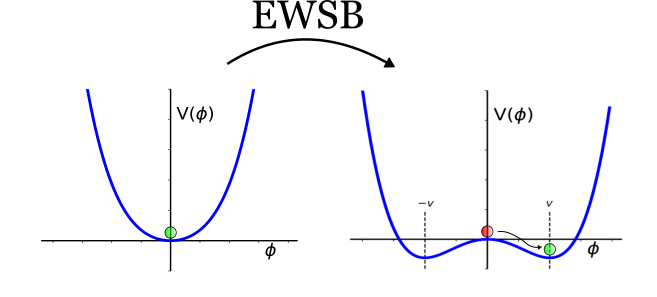
\includegraphics[width=0.75\textwidth]{figures/chapter1/higgs_potential_trans}
		\caption{Illustration of electroweak symmetry breaking (EWSB).
			\textbf{\textit{Left}}: Higgs potential with $\mu^2>0$ with stable equilibrium at $\phi=0$.
			\textbf{\textit{Right}}: With $\mu^2<0$, $\phi=0$ is no longer
			a stable equilibrium and the Higgs attains a non-zero vacuum
			expectation value at $\pm v$ --- breaking the \SUewk~gauge symmetry of the electroweak
			sector of the SM.
		}
	\label{fig:higgs_ewsb}
	\end{center}
\end{figure}

As opposed to `eating' gauge degrees of freedom as in the case of the \fieldWpm~and \fieldZ~bosons,
the fermion masses are obtained by adding additional interaction terms to \SML~between the
fermions and Higgs fields,
\begin{align}
	\mathcal{L}_{f-h} = y_f \left( \bar{L} \phi e^-_R + \phi^{\dagger} \overline{e^-}_R L\right).
	\label{eq:higgs_fermion_int}
\end{align}
Since both $L$ and $\phi$ are \SUtwo~doublets, adding the right-handed \SUtwo~singlet terms
do not spoil the \SUtwo~symmetry.
When the Higgs field acquires a non-zero vev after EWSB, we can insert Equation~\ref{eq:higgs_perturb} into Equation~\ref{eq:higgs_fermion_int} to obtain expressions for the fermions masses,
\begin{align}
	m_f = y_f \frac{v}{\sqrt{2}},
	\label{eq:fermion_mass_term}
\end{align}
where the $y_f$ are referred to as the fermion \textit{Yukawa couplings}, and are free parameters
of the SM that need to be measured.
Additional interactions arise between the fermions and $h(x)$ whose couplings are related
to the fermion masses as,
\begin{align}
	\mathcal{L}_{f-h} \propto \frac{m_f}{v} \bar{f}f h.
	\label{eq:higgs_fermion_coupling}
\end{align}

The general form Equation~\ref{eq:higgs_fermion_int} implies that the $y_f$ are matrices representing the
Higgs-fermion Yukawa couplings. They can be diagonalized by performing the proper unitary
transformations between the weak- and mass-bases of the fermion fields. In the case of the leptons,
this rotation is the identity: the lepton's weak eigenbasis is the same as their mass eigenbasis.
This is mainly due to the extraordinarily large mass difference between the charged and neutral
leptons within each lepton generation~\cite{Akhmedov:2007fk}. Within the quark-sector,  however,
the mass- and weak-basis fermion fields differ. This implies that the diagonalization procedure results
in mixing among the weak eigenstates of the quark fields to produce the observed mass eigenstates; i.e. the quark mass-eignstates ($d$,
$s$, $b$) are
coherent mixtures of the weak eigenstates ($d^{\prime}$,
$s^{\prime}$, $b^{\prime}$).\footnote{The mixing can be parametrised as either occurring between
the up-type, down-type, or a mixture of up- and down-type fields of each \SUtwo~doublet. Without
loss of generality and for simplicity, it is usually given with respect to the down-type quark fields as shown
here.}
This allows for the flavor-changing processes that are present
in charged weak interactions, allowing for interaction terms involving the decay
of a quark of one family into that of another family. The amount of mixing in the quark sector
is dictated by a $3\times 3$ unitary matrix known as the \textit{Cabibbo-Kobayashi-Maskawa} (CKM)
matrix~\cite{Kobayashi:1973fv} $\mathcal{V}_{\text{CKM}}$, the general form of which has four free parameters: three mixing angles
and a complex phase, $\delta$. The off-diagonal terms of the CKM matrix and the value of the mixing angles
dictate the amount of flavor mixing in the quark sector. The complex phase $\delta$
allows for charge-parity (CP) symmetry violating effects to occur. In fact, this term is the \textit{only} term of the SM
that allows for CP-violation --- an effect important for providing interactions that are asymmetric
between matter and anti-matter fields.\footnote{Charge Parity (CP) symmetry refers to the invariance
	of a theory with respect to swapping particles with their corresponding anti-particles and, additionally,
	inverting a field's spatial coordinates, $\psi(\vec{x}) \rightarrow \psi(-\vec{x})$. The former
	is the `C' symmetry and the latter is the `P' symmetry.
}

The remaining terms of $V(\phi)$ (Equation~\ref{eq:higgs_potential}) involve only the Higgs field. After
EWSB and the Higgs field acquiring vev we obtain,
\begin{align}
	V(\phi) \rightarrow V(\phi)_{\text{EWSB}} =  -\lambda \nu^2 h^2 - \lambda \nu h^3 - \frac{1}{4} \lambda h^4 + \text{const.}
	\label{eq:higgs_potential_self_int}
\end{align}
where we have ignored the terms already discussed above. The first term of Equation~\ref{eq:higgs_potential_self_int}
is the Higgs boson mass term, the second and third are the triple and quartic Higgs self-couplings,
\begin{align}
	\underbrace{m_{h} = \sqrt{ - 2 \mu^2} = \sqrt{ 2 \lambda v^2 }}_\text{Higgs boson mass} \hspace{1cm} \underbrace{\mathcal{L}_{hhh} \propto \frac{m_h^2}{v} \hspace{1cm} \mathcal{L}_{hhhh} \propto \frac{m_h^2}{v^2}}_\text{Triple and quartic Higgs self-couplings}.
	\label{eq:higgs_self_couplings}
\end{align}





%%%%%%%%%%%%%%%%%%%%%%%%%%%%%%%%%%%%%%%%%%%
%%%%%%%%%%%%%%%%%%%%%%%%%%%%%%%%%%%%%%%%%%%
%% sub section describing the standard model finally and its successes
%%%%%%%%%%%%%%%%%%%%%%%%%%%%%%%%%%%%%%%%%%%
%%%%%%%%%%%%%%%%%%%%%%%%%%%%%%%%%%%%%%%%%%%
%\section{The Complete Standard Model, Successes and Shortcomings}
\label{sec:final_sm_description}

The physical field content of the SM, after EWSB, is detailed in Table~\ref{tab:sm_content_EWSB}
Also shown in Table~\ref{tab:sm_content_EWSB} are the electric charge associated with each
particle field, $Q$, the relevant couplings, and particle masses.


\begin{table}[!htb]
    \caption{
        The table shows the particle fields of the SM after SSB. Coupling and mass parameters are provided. 
    }
        %The particle content of the SM after the process of
        %electroweak symmetry breaking.
        %Shown for each particle species are the associated electric charge, $Q$,
        %coupling, and mass (approximate).
        %The $y_i$ are the Yukawa coupling (Equation~\ref{eq:higgs_fermion_coupling}),
        %$\alpha_{\text{EM}}$ is the QED coupling constant (`fine structure constant'),
        %$\mathcal{V}$ indicates the parameters of the CKM matrix, and
        %$\alpha_s$ is the QCD coupling constant.
        %The quantities $\lambda$ and $\mu$ are the Higgs self-coupling parameter
        %and mass terms, respectively, appearing in Higgs potential terms (Equation~\ref{eq:higgs_potential}).
    \begin{center}
        \begin{tabularx}{1\textwidth}{m{1em} c c c c }
        \toprule
        \hline
        & Physical Field & Q & Coupling & Mass [GeV] \\
        \hline
        \rotatebox{90}{\hspace{-0.1cm}\textbf{Quarks} } 
            & \makecell{ \quarkU, \quarkC, \quarkT \\ \quarkD, \quarkS, \quarkB} % FIELD
            & \makecell{ $2/3$ \\ $-1/3$ }% Q
            %& \makecell{ $\mathbf{3}$ \\ $\mathbf{3}$ } % SU(3)
            & \makecell{ ($y_i=$) $1\times10^{-5}$, $7\times10^{-3}$, $1$ \\ ($y_i=$) $3\times10^{-5}$, $5\times10^{-4}$, $0.02$ } % Coupling
            & \makecell{ $2\times10^{-3}$, $1.27$, $173$ \\ $4\times10^{-4}$, $0.10$, $4.18$ }\\% Mass
        \rotatebox{90}{\hspace{-0.1cm}\textbf{Leptons} } 
            & \makecell{ \leptonE, \leptonMu, \leptonTau \\ \neutrinoE, \neutrinoMu, \neutrinoTau } % FIELD
            & \makecell{ $-1$ \\ $0$ }% Q
            %& \makecell{ $\mathbf{1}$ \\ $\mathbf{1}$ } % SU(3)
            & \makecell{ ($y_i=$) $3\times10^{-7}$, $6\times10^{-4}$, $0.01$ \\ -- } % Coupling
            & \makecell{ $5\times10^{-4}$, $0.106$, $1.777$ \\ --}\\% Mass
        \midrule
        \rotatebox{90}{\textbf{Bosons} } 
            & \makecell{ \fieldPhoton \\ \fieldZ \\ (\fieldWp, \fieldWm) \\ \fieldG } % FIELD
            & \makecell{ $0$ \\ $0$ \\ $(+1,-1)$ \\ $0$ }% Q
            %& \makecell{ $\mathbf{1}$ \\ $\mathbf{1}$ \\ $\mathbf{1}$ \\ $\mathbf{8}$ } % SU(3)
            & \makecell{ $\alpha_{\text{EM}} \simeq 1/137$ \\ $\sin \theta_{W} \simeq 0.5$ \\ $\mathcal{V}_{\text{CKM}}$ \\ $\alpha_s \simeq 0.1$ } % Coupling
            & \makecell{ $0$ \\ $91.2$ \\ $80.4$ \\  $0$}\\% Mass
        \midrule
        \rotatebox{90}{\textbf{Higgs} } 
            & \makecell{ \fieldH } % FIELD
            & \makecell{ $0$ }% Q
            %& \makecell{ $\mathbf{1}$ } % SU(3)
            & \makecell{ $\lambda$, $\mu$ } % Coupling
            & \makecell{ $125.09$ }\\% Mass
        \hline
        \bottomrule
        \end{tabularx}
    \end{center}
    \label{tab:sm_content_EWSB}
\end{table}


%%%%%%%%%%%%%%%%%%%%%%%%%%%%%%%%%%%%%%%%%%%%%%%%%%%%%%%%%%%%%%%%%%%%%%%%%%%%%%%%%
%%%%%%%%%%%%%%%%%%%%%%%%%%%%%%%%%%%%%%%%%%%%%%%%%%%%%%%%%%%%%%%%%%%%%%%%%%%%%%%%%
%%%%%%%%%%%%%%%%%%%%%%%%%%%%%%%%%%%%%%%%%%%%%%%%%%%%%%%%%%%%%%%%%%%%%%%%%%%%%%%%%
%
% SUCCESSES
%
%%%%%%%%%%%%%%%%%%%%%%%%%%%%%%%%%%%%%%%%%%%%%%%%%%%%%%%%%%%%%%%%%%%%%%%%%%%%%%%%%
%%%%%%%%%%%%%%%%%%%%%%%%%%%%%%%%%%%%%%%%%%%%%%%%%%%%%%%%%%%%%%%%%%%%%%%%%%%%%%%%%
%%%%%%%%%%%%%%%%%%%%%%%%%%%%%%%%%%%%%%%%%%%%%%%%%%%%%%%%%%%%%%%%%%%%%%%%%%%%%%%%%

\subsection{Successes of the Standard Model}
\label{sec:sm_successes}

The particle content presented in Table~\ref{tab:sm_content_EWSB} represents the current
picture of the visible matter content of the Universe.
It is a concise picture.
With this particle content in hand, and the description of their fundamental particle interactions (Equation~\ref{eq:sm_lagrangian}),
the predictive power of the SM is immense.

Figure~\ref{fig:sm_xsec_summary} shows a summary of LHC measurements of cross-sections
for various production processes at 7, 8, and 13\,TeV.
The agreement of these measurements with the theoretical predictions provided by the SM, spanning over 10 orders of magnitude,
is an incredible testament to the power of the SM and the toolkit provided by QFT.
The power of the SM, and its internal consistency, is illustrated in Figure~\ref{fig:mw_mt_scan},
which shows the results of indirect measurements of the $W$-boson and top-quark masses based
on fits to electroweak precision data.
When all measurements other than those on $m_h$ are included, the constraints of the SM
only allow for a small region of the $(m_{\text{top}}, M_W)$ parameter space.
Adding the Higgs mass measurement results only shrinks this allowed area.
The fact that these indirect measurements agree so well with the direct measurements paints a picture
of the SM as being a fundamentally complete picture of the known physical phenomena.
It is likely that if the SM were not accounting for particular types of interactions or fields,
the level of agreement between the direct measurements and those obtained indirectly via
fits to electroweak precision data would not be to the level seen in Figure~\ref{fig:mw_mt_scan}.

\begin{figure}[!htb]
    \begin{center}
        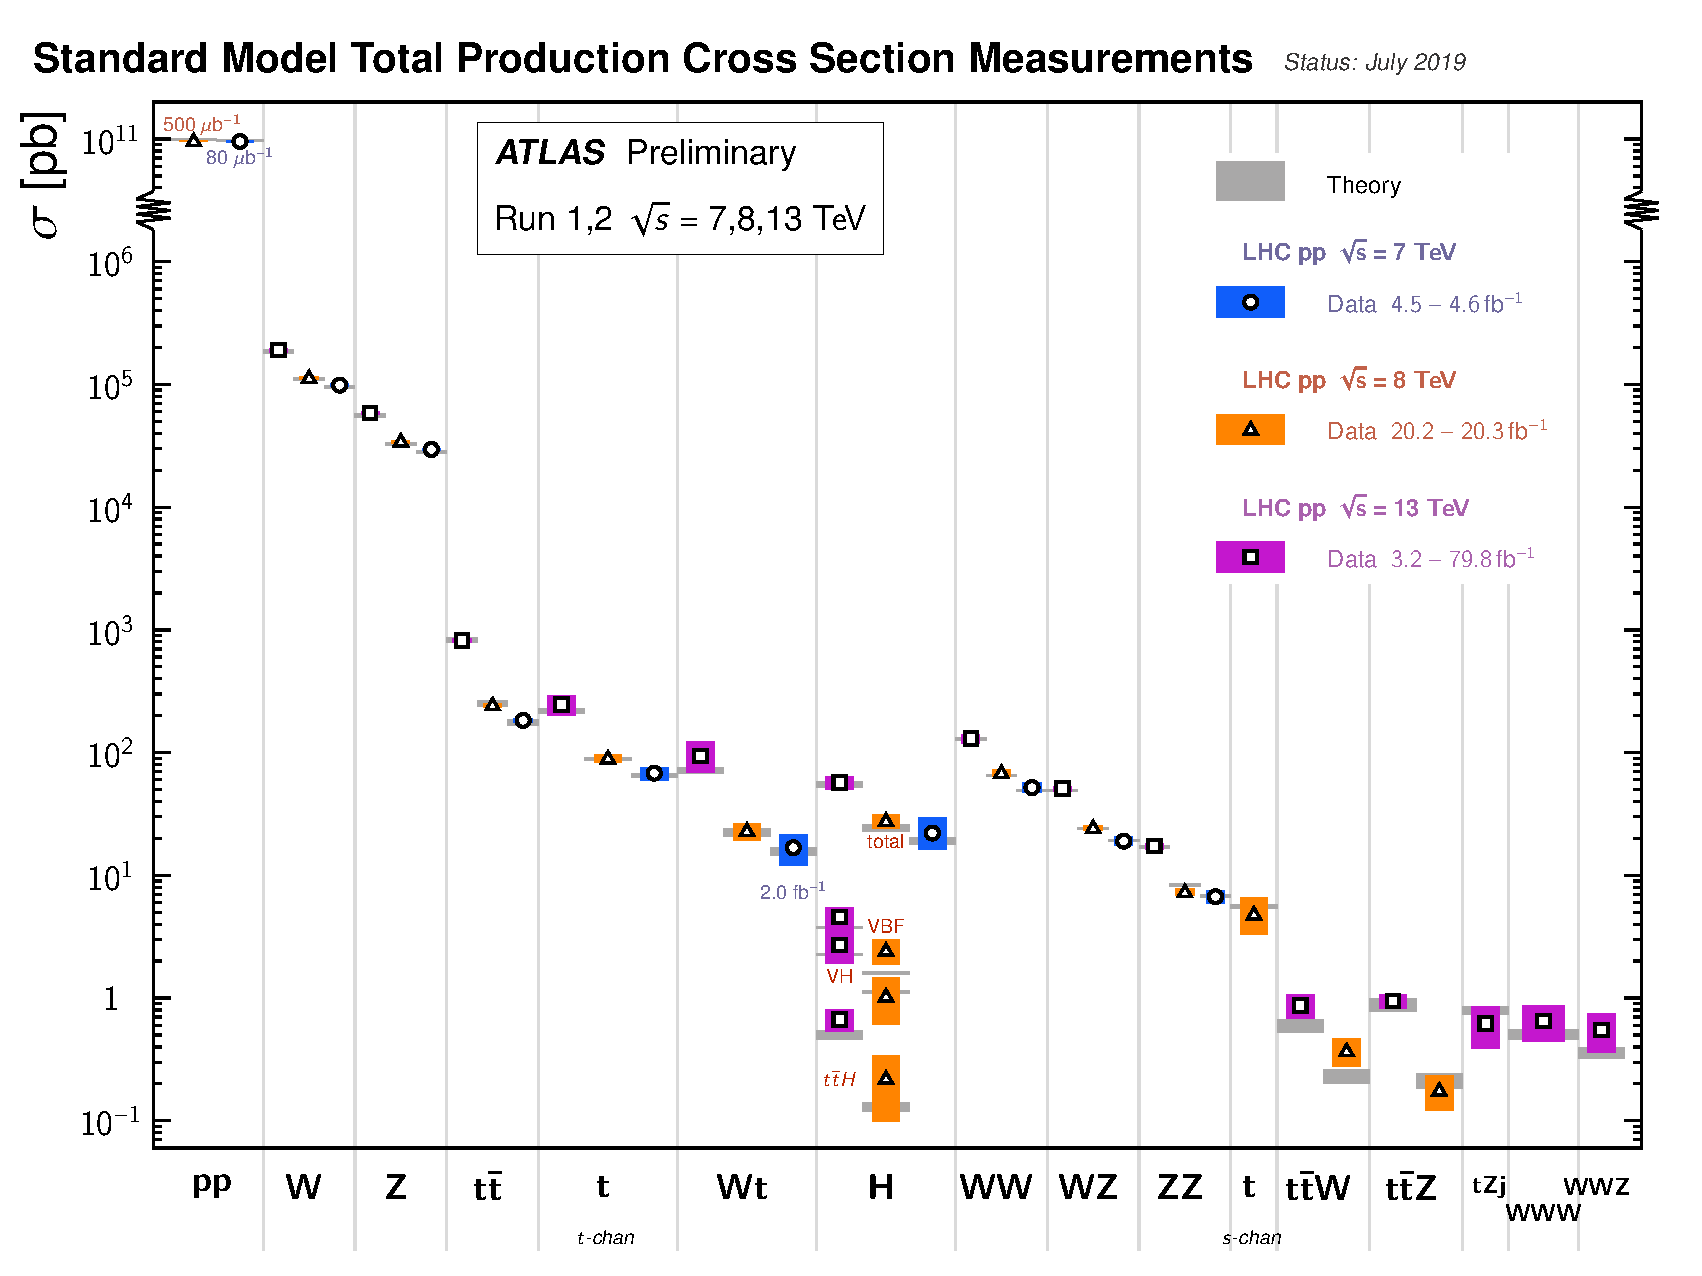
\includegraphics[width=0.75\textwidth]{figures/chapter1/sm_final/sm_xsec_summary}
        \caption{
            summary of several standard model total production cross section measurements,
            corrected for branching fractions, compared to the corresponding theoretical expectations. 
            figure taken from ref.~\cite{smsummaryxsec}.
        }
        \label{fig:sm_xsec_summary}
    \end{center}
\end{figure}
\begin{figure}[!htb]
    \begin{center}
        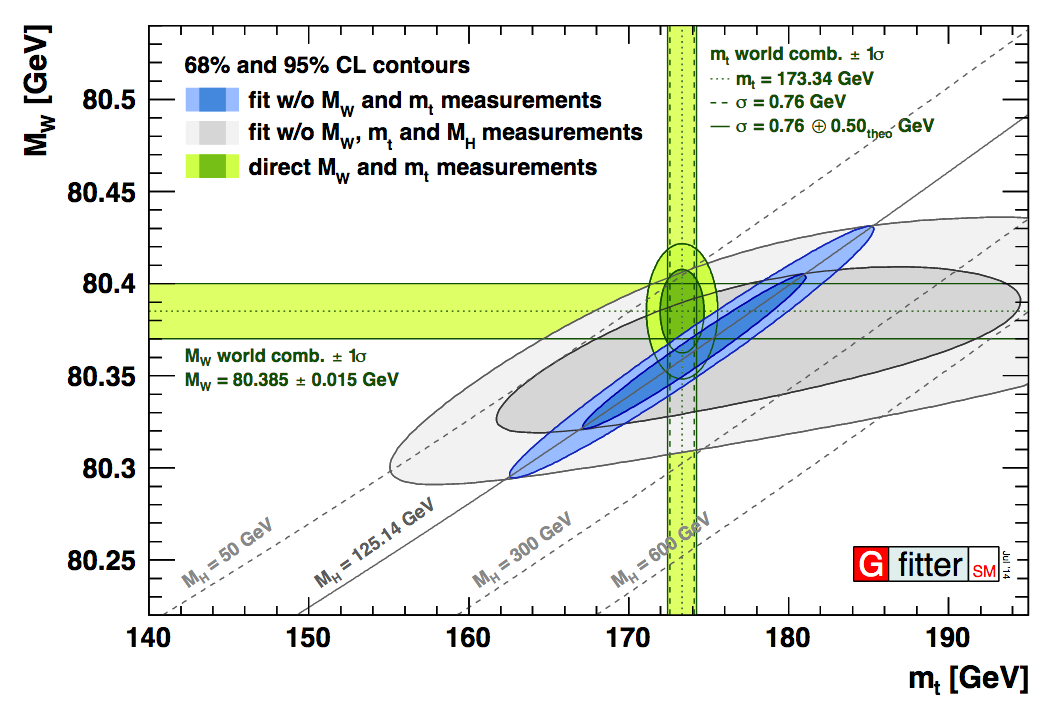
\includegraphics[width=0.65\textwidth]{figures/chapter1/sm_final/mw_vs_mt_indirect}
        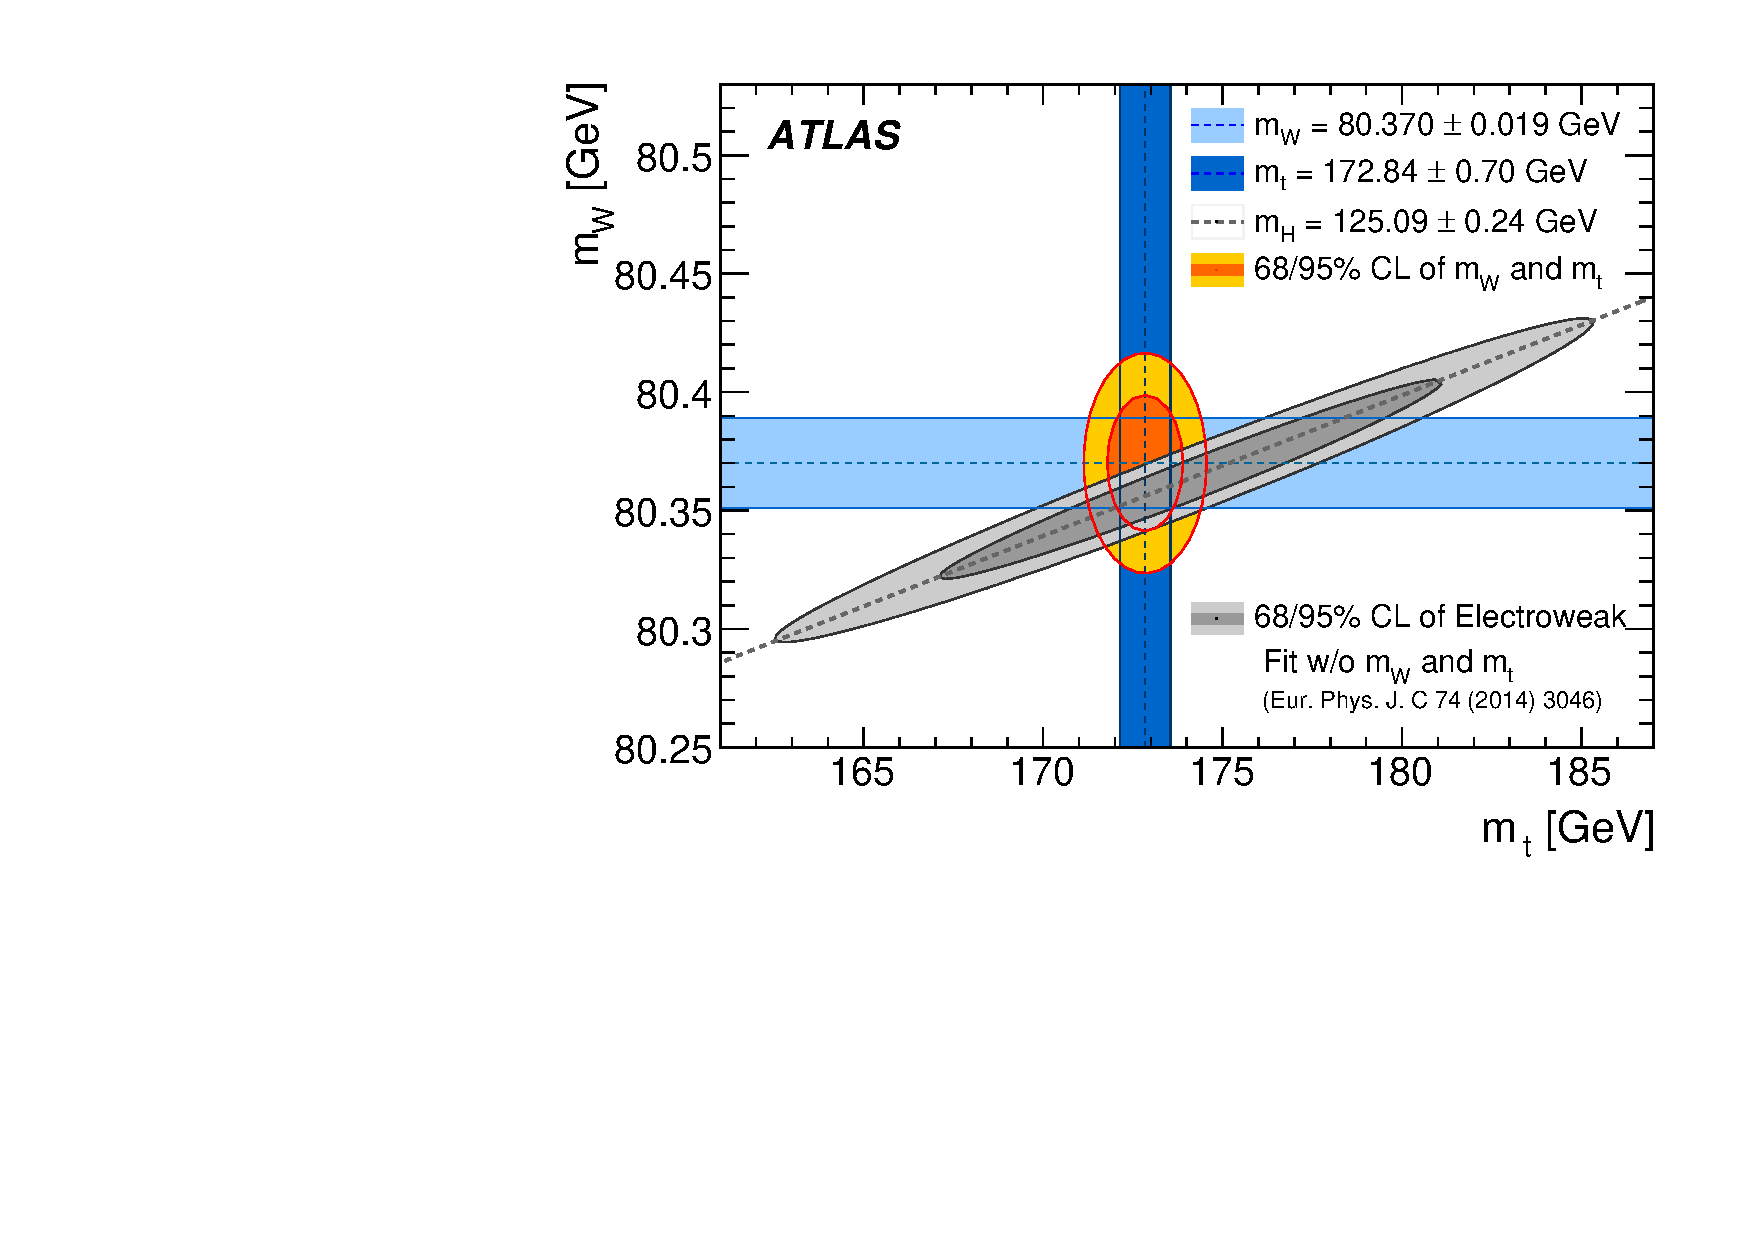
\includegraphics[width=0.69\textwidth]{figures/chapter1/sm_final/atlas_w_boson_mass_mw_mt}
        \caption{
            Contours at 68\% and 95\% CL obtained from scans of $M_W$ versus $m_{\text{top}}$,
            for the global electroweak fits in comparison to the direct measurements.
            \textit{\textbf{Top}}: Including Higgs boson mass measurements in the indirect fit~\cite{HMassATLAS,HMassCMS} (blue)
                or excluding them (grey). Figure taken from Ref.~\cite{GFitter}.
            \textit{\textbf{Bottom}}: Including the latest precision $W$-boson mass measurement from the ATLAS
                experiment. Figure taken from Ref.~\cite{ATLASWMass}.
        }
        \label{fig:mw_mt_scan}
    \end{center}
\end{figure}

With the discovery a Higgs boson like particle with a mass at 125\,GeV in 2012~\cite{HDiscoveryATLAS,HDiscoveryCMS},
the final piece of the SM described by Equation~\ref{eq:sm_lagrangian} is potentially found.
The 2012 Higgs discovery meant the start of a very long experimental program, focused
on studying this new particle and confirming its role as being the fundamental scalar boson, $\phi$,
appearing in the SM.

It should be stressed that the terms associated with the Higgs potential appearing in the SM
Lagrangian, given by Equation~\ref{eq:higgs_potential}, are by no means fundamental.
They do not have to appear in this way.
The terms appearing in Equation~\ref{eq:higgs_potential} take the form they do since they
could lead to masses for the fermions and gauge bosons.
There is no fundamental symmetry motivating their precise form.
The BEH mechanism is inspired by that of super-conductivity, in which the formation of composite (i.e. not elementary)
scalar particles --- the Cooper pairs --- occurs.
The fact that the same type of phase transition should describe the generation of masses for
the elementary particles of the SM, and that it should presuppose the existence of an \textit{elementary}
scalar boson, was simply left as one of the last open questions of the SM.
In a sense, the truth of the form underlying Equation~\ref{eq:higgs_potential} was not important to BEH.
The more important takeaway was that there \textit{could} be a mechanism by which the SM particles acquired
mass without disrupting the fundamental gauge structure of the SM that had already held up to experimental scrutiny.

It is then up to the experiments to verify that the 125\,GeV scalar boson discovered in 2012
is responsible for the BEH mechanism as described in Section~\ref{sec:higgs_description}.
The form of the Higgs potential as defined in Equation~\ref{eq:higgs_potential} makes
very clear predictions on the form and strengths of the couplings to the known fundamental particles:
the gauge bosons and fermions, with couplings to the Higgs predicted to take the forms
of Equations~\ref{eq:higgs_gauge_couplings} and \ref{eq:higgs_fermion_coupling}, respectively.
It is then up to the ATLAS and CMS experiments to verify that the new particle couples
to these `old' particles just as predicted.
The coupling strengths also dictate the Higgs decay rates into specific SM particles, as indicated
in Figure~\ref{fig:higgs_br_sm}.
Any deviation with respect to the SM-predicted values in the measurement of the Higgs decay branching ratios, or
in the values of the fermion or gauge coupling strengths and their dependence on the
particle masses, would indicate that the particle discovered in 2012 is not the Higgs boson as predicted
in the SM.

All of the measurements of the properties of the 125 GeV particle
made by the ATLAS and CMS experiments are so far in fairly good agreement with the SM prediction
of a $m_h = 125$ GeV Higgs boson~\cite{HProp0,HProp1,HProp2,HProp3,HProp4,HProp5,HProp6,HProp7,HProp8}.
The agreement with the SM prediction, over a wide variety of measurements, is illustrated in
Figure~\ref{fig:higgs_measurements} which shows the measurements of the fermion and gauge
couplings and of the cross-sections of the leading Higgs production mechanisms and decay
branching ratios.
Within the precision of these measurements, the SM is fully supported by the experiments
and it appears as though the particle discovered in 2012 is in fact the particle as predicted
by BEH.

\begin{figure}[!htb]
    \begin{center}
        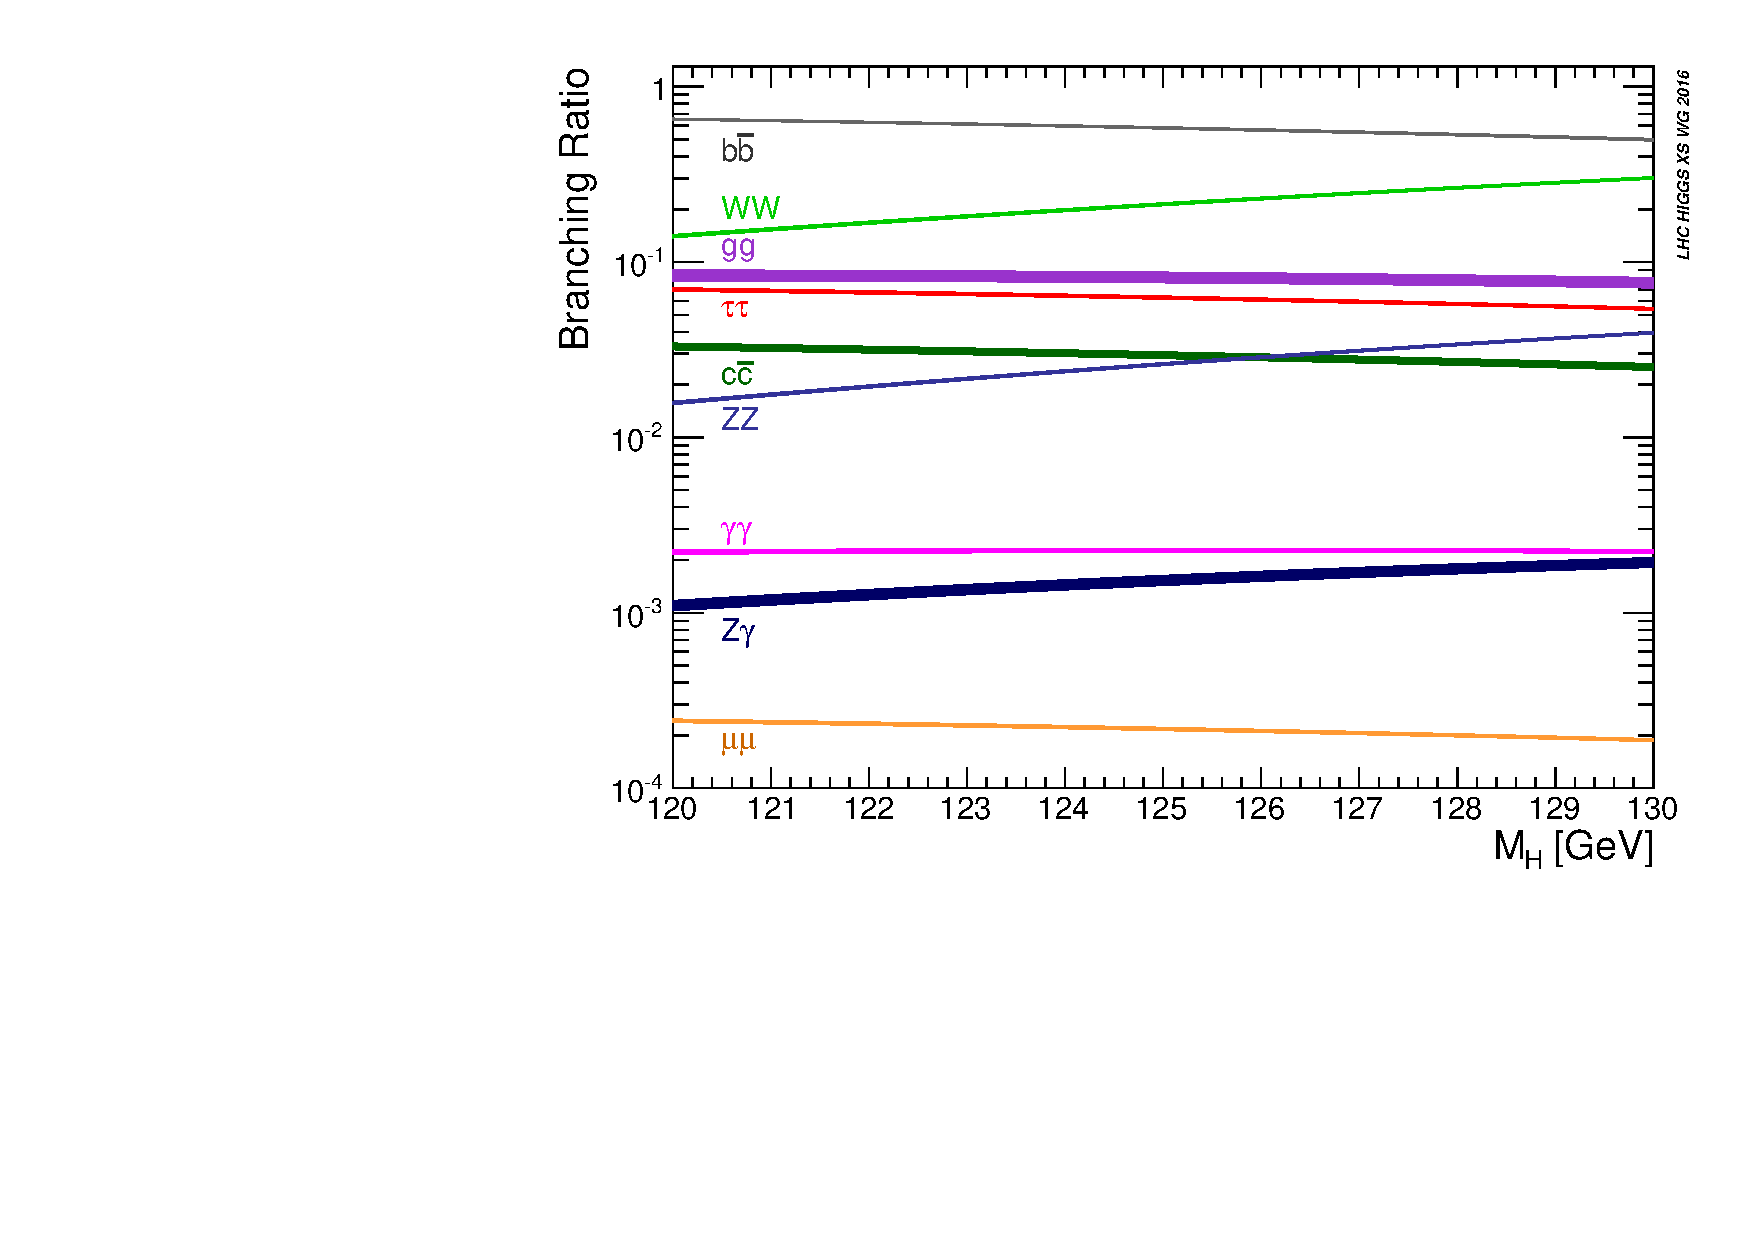
\includegraphics[width=0.6\textwidth]{figures/chapter1/sm_final/higgs_br_sm}
        \caption{
            Predicted branching ratios for an SM-like Higgs boson with $m_{h} = 125\,\GeV$.
            Figure taken from Ref.~\cite{deFlorian:2016spz}.
        }
        \label{fig:higgs_br_sm}
    \end{center}
\end{figure}

\begin{figure}[!htb]
    \begin{center}
        \raisebox{1cm}{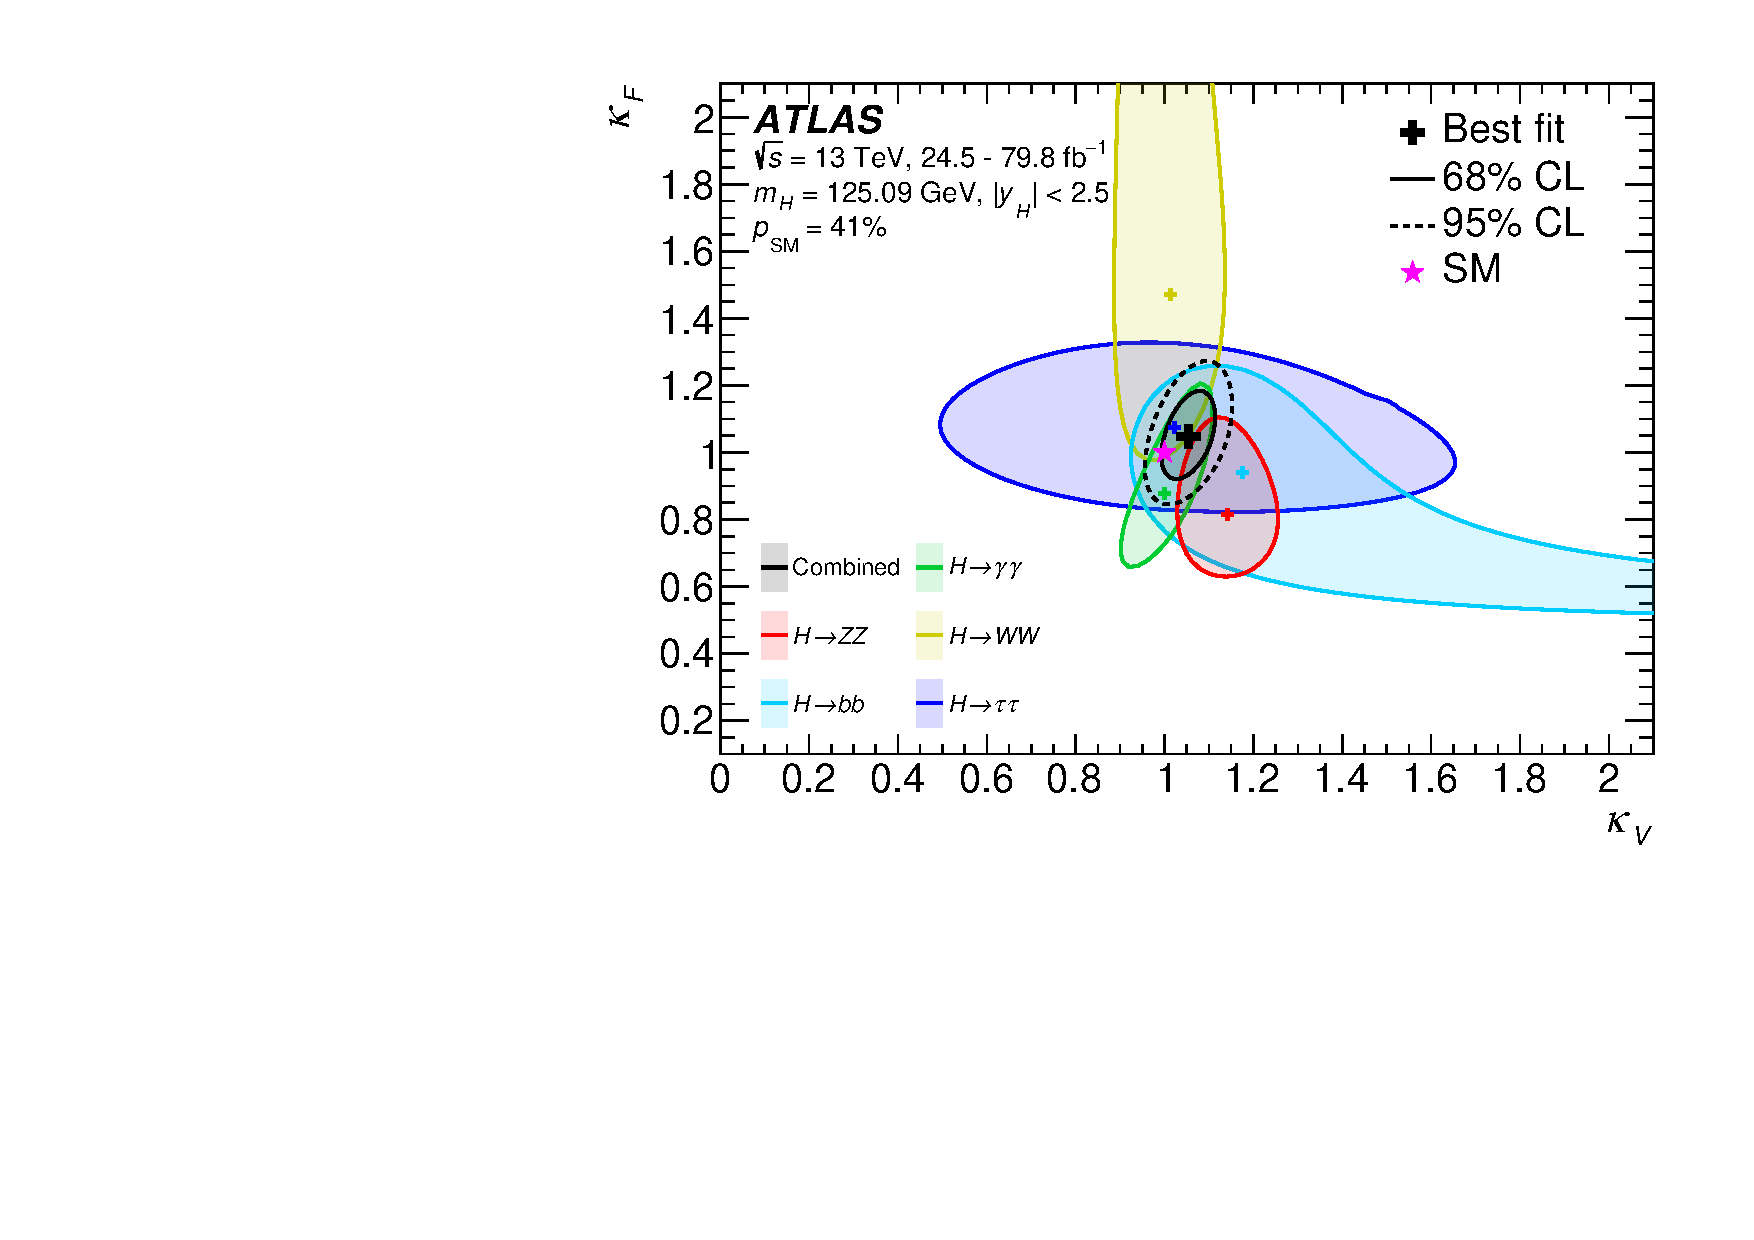
\includegraphics[width=0.49\textwidth]{figures/chapter1/sm_final/higgs_kappa_v_f}}
        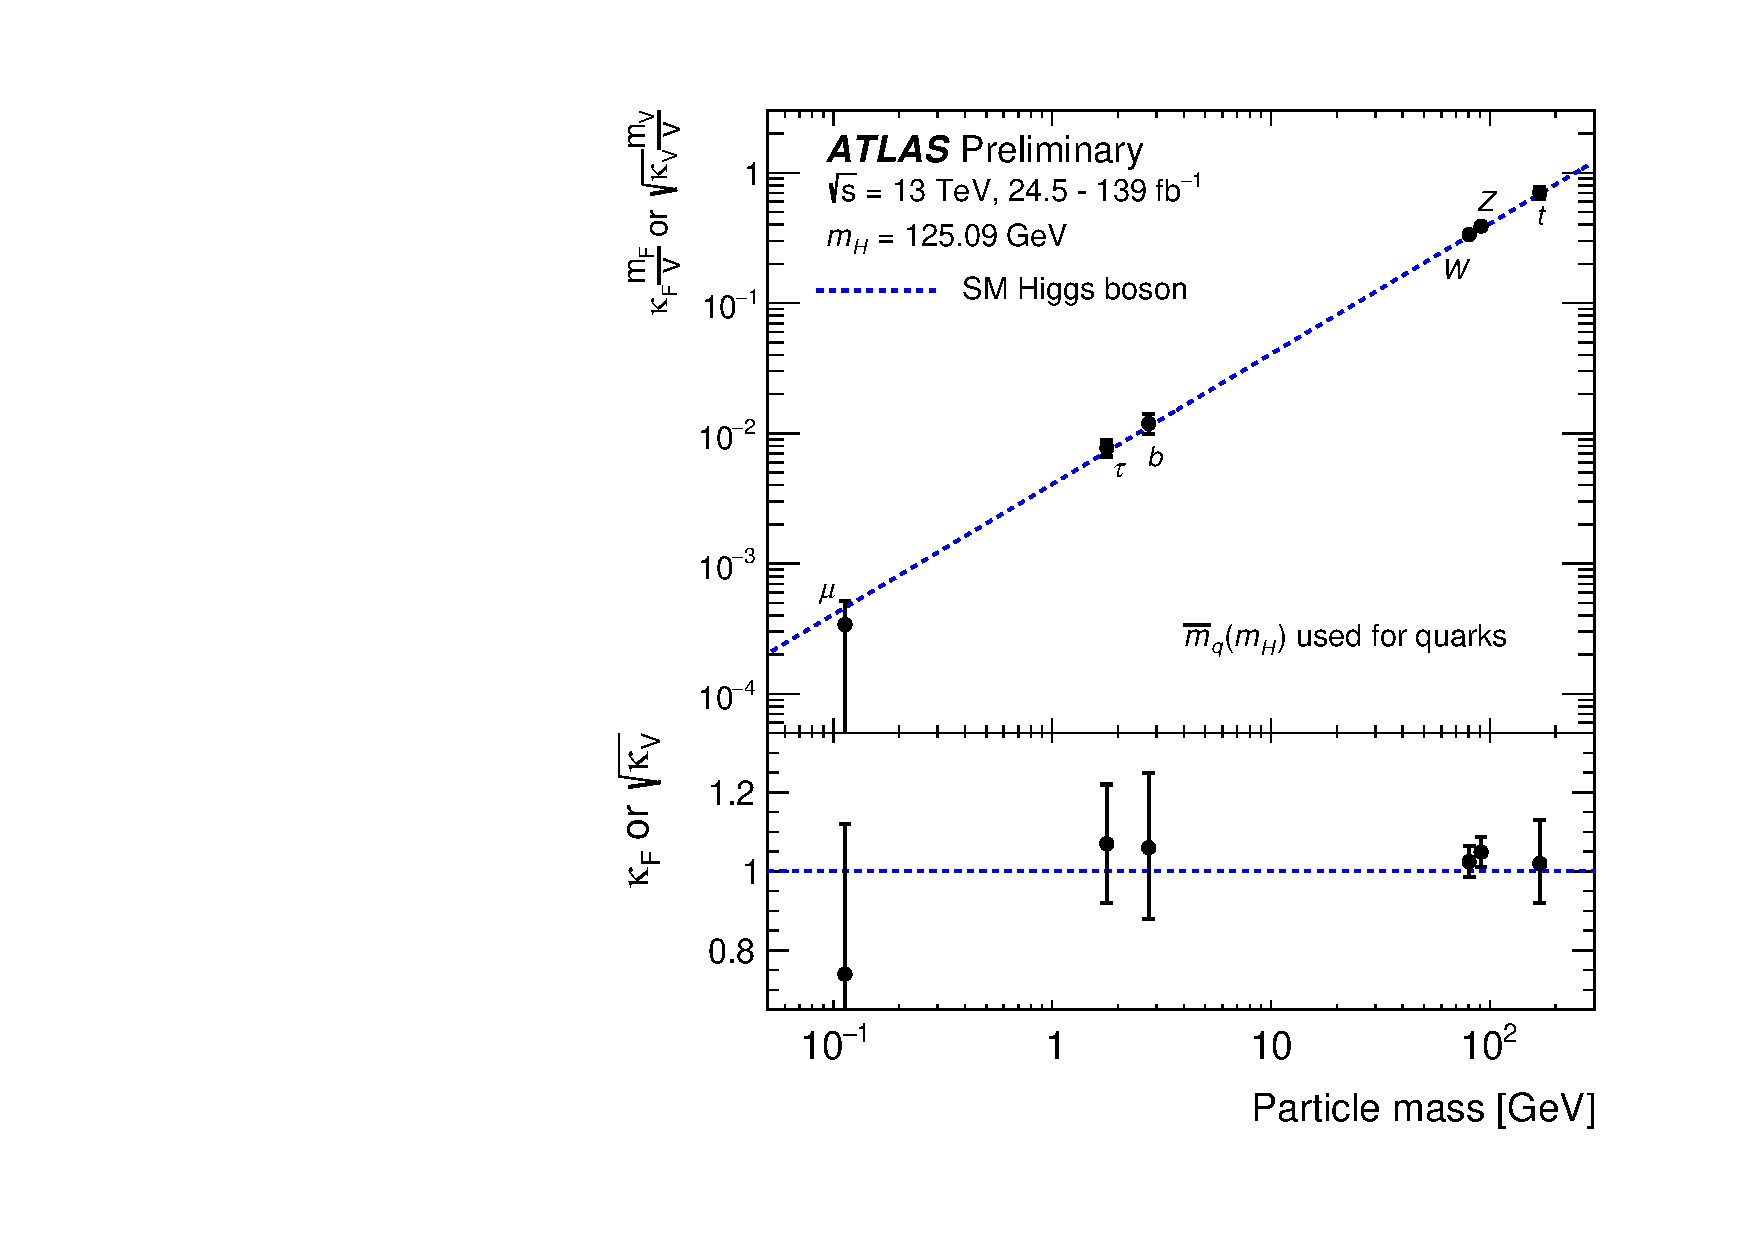
\includegraphics[width=0.49\textwidth]{figures/chapter1/sm_final/higgs_kappa_vs_mass}
        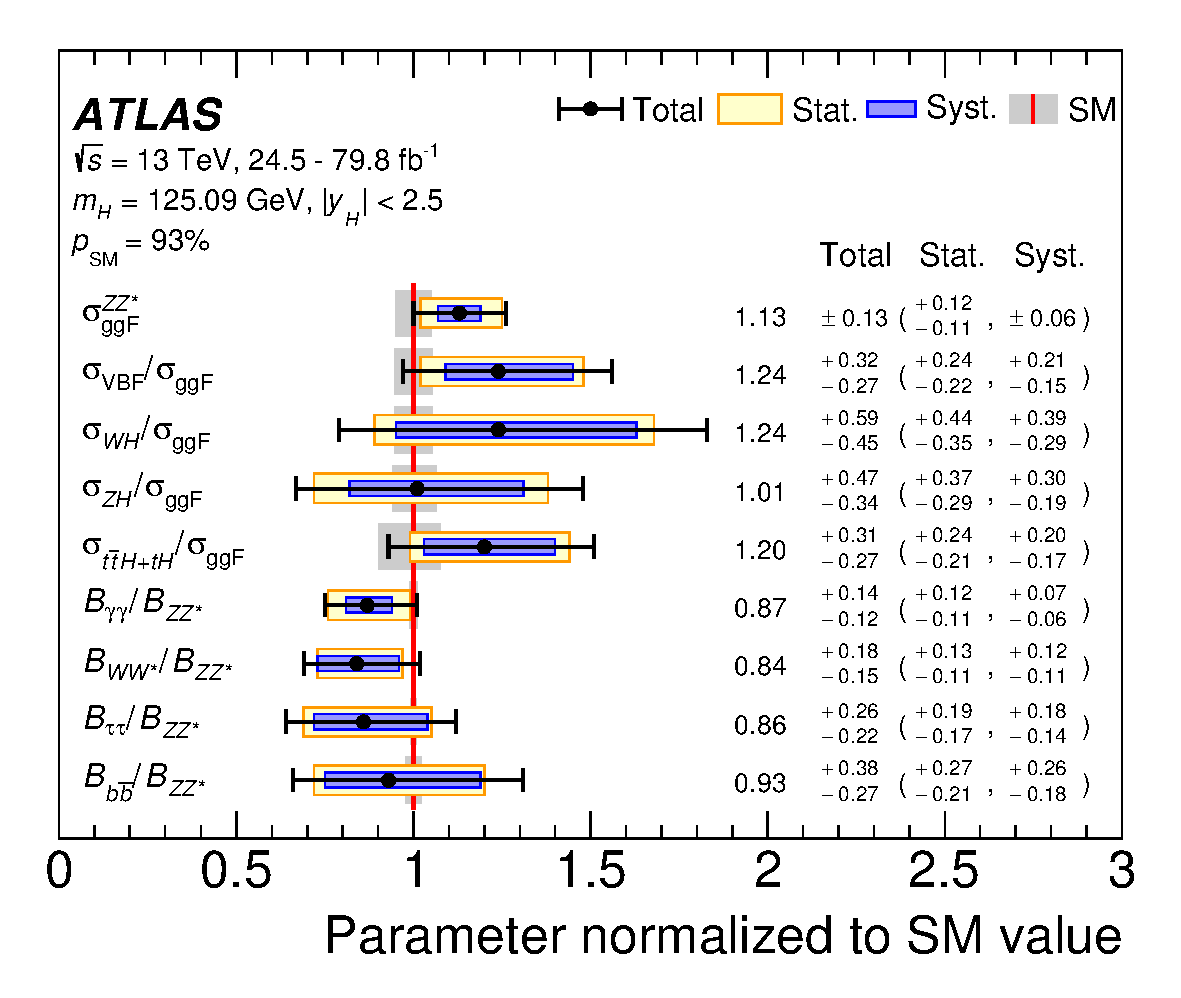
\includegraphics[width=0.49\textwidth]{figures/chapter1/sm_final/higgs_prod_and_br}
        \caption{
            Higgs precision measurements of couplings to SM particles.
            Figures taken from Ref.~\cite{HiggsProps}.
            \textit{\textbf{Left}}: Combined measurement of fermion and gauge-boson Higgs coupling modifiers, $\kappa_f$
                and $\kappa_V$ (assumed to be universal across fermion and gauge-boson species in the result pictured).
                Values of $\kappa_f$ or $\kappa_V$ equal to 1 correspond to the SM prediction for the Higgs' couplings to
                these particles.
            \textit{\textbf{Right}}: Measured values of the Higgs fermion and gauge-boson coupling parameters
                as a function of the fermion and gauge-boson masses.
                The blue dashed line shows the SM prediction (Equations~\ref{eq:higgs_gauge_couplings} and \ref{eq:higgs_fermion_coupling}).
            \textit{\textbf{Bottom}}: Measurements of Higgs production cross sections and (relative) decay branching ratios.
        }
        \label{fig:higgs_measurements}
    \end{center}
\end{figure}

In addition to the Higgs couplings to the SM fermions and gauge bosons, the SM Lagrangian
predicts terms describing the Higgs \textit{self}-couplings.
These terms are described by the $\lambda$ parameter in Equation~\ref{eq:higgs_potential}
and appearing in Table~\ref{tab:sm_content_EWSB}.
The Higgs self-coupling parameter $\lambda$ has a value predicted by the SM, as seen in 
Equation~\ref{eq:higgs_self_couplings}, which is fixed by the Higgs boson mass.
The parameter $\lambda$ is directly responsible for providing the structure of the Higgs potential,
indicated by Equation~\ref{eq:higgs_potential_self_int}, and therefore plays a fundamental
role in EWSB.
Measuring how the 125\,GeV Higgs boson couples and decays to the SM fermions and gauge bosons,
then, is only a necessary requirement for confirming that the particle is the one predicted by
the SM: it is not sufficient.
To truly confirm that the 125\,GeV boson is indeed that predicted by the SM, and that EWSB
is described by the BEH mechanism, the Higgs self-coupling parameter will have to be measured
experimentally and confirmed to take its predicted value given by Equation~\ref{eq:higgs_self_couplings}.

Direct measurement of $\lambda$ proceeds only through the observation of events in which Higgs bosons
are produced in pairs.
At the LHC, this process occurs predominantly via gluon-gluon fusion through the two diagrams illustrated
in Figure~\ref{fig:hh_feynman}.
The triangle and box diagrams shown in Figure~\ref{fig:hh_feynman} represent destructively interfering amplitudes.
As a result, the cross-section associated with the production of Higgs boson pairs is exceedingly low
and statistically significant observation of this process is not expected to occur until
near the end of the lifetime of the LHC.
The study of Higgs boson pairs is the subject of the analysis to be presented in Chapter~\ref{chap:search_hh}.

\begin{figure}[!htb]
    \begin{center}
        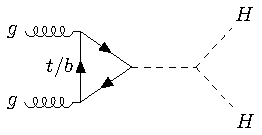
\includegraphics[width=0.7\textwidth]{figures/search_hh/feynman_diagrams/fdiagram_triangle}
        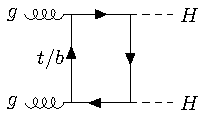
\includegraphics[width=0.55\textwidth]{figures/search_hh/feynman_diagrams/fdiagram_box}
        \caption{
            Representative Feynman diagrams that contribute at leading order in QCD to the non-resonant
            production of Higgs boson pairs.
            {\textbf{\textit{Top}}}: The `triangle' diagram, sensitive to the Higgs self-coupling, $\lambda$.
            {\textbf{\textit{Bottom}}}: The `box' diagram, sensitive to the (squared) Yukawa couplings to the third generation
            fermions entering the loop.
        }
        \label{fig:hh_feynman}
    \end{center}
\end{figure}

%%%%%%%%%%%%%%%%%%%%%%%%%%%%%%%%%%%%%%%%%%%%%%%%%%%%%%%%%%%%%%%%%%%%%%%%%%%%%%%%%
%%%%%%%%%%%%%%%%%%%%%%%%%%%%%%%%%%%%%%%%%%%%%%%%%%%%%%%%%%%%%%%%%%%%%%%%%%%%%%%%%
%%%%%%%%%%%%%%%%%%%%%%%%%%%%%%%%%%%%%%%%%%%%%%%%%%%%%%%%%%%%%%%%%%%%%%%%%%%%%%%%%
%
% SHORTCOMINGS
%
%%%%%%%%%%%%%%%%%%%%%%%%%%%%%%%%%%%%%%%%%%%%%%%%%%%%%%%%%%%%%%%%%%%%%%%%%%%%%%%%%
%%%%%%%%%%%%%%%%%%%%%%%%%%%%%%%%%%%%%%%%%%%%%%%%%%%%%%%%%%%%%%%%%%%%%%%%%%%%%%%%%
%%%%%%%%%%%%%%%%%%%%%%%%%%%%%%%%%%%%%%%%%%%%%%%%%%%%%%%%%%%%%%%%%%%%%%%%%%%%%%%%%
\FloatBarrier
\subsection{Perceived Shortcomings of the Standard Model and Open Questions}
\label{sec:sm_shortcomings}

Despite the impressive results and predictive power of the SM illustrated in the previous
section, the SM is unable to provide a complete picture of what we now consider the observed
Universe.
A few items that are clearly not explained within the framework of the SM are described below.
%A few items that are clearly not explainable under the framework of the SM are described below.
Chapter~\ref{chap:bsm} goes on to introduce an extension to the SM that provides explanations
for many of these short comings of the SM.

\begin{description}
    \item[] \textbf{Existence of Dark Matter (DM) and Dark Energy (DE)} \\
        Most of the experimental evidence that we currently have that supports the notion that
        physics beyond the SM (BSM) exists comes not from collider-based particle physics experiments,
        but from astrophysical observations.
        Astrophysical observations suggest that the majority of the matter content of the Universe
        is composed of a non-luminous, weakly interacting type of matter referred to as `Dark Matter' (DM)
        and that the expansion of the Universe is accelerating, perhaps due to presence of
        `Dark Energy' (DE)~\cite{Davis:2014csa,PlanckCollab}.
        There has not yet been experimental proof of the particle nature of DM, but
        many theories suggest that it fall under the class of `Weakly Interacting Massive Particle' (WIMPs), i.e. that it be `WIMP-like'.
        The particle nature of DE is completely unknown and without a fundamental description.
    \item[] \textbf{Massive Neutrinos} \\ The observation of neutrino oscillations~\cite{Fukuda:1998mi} provides evidence
        in support of neutrinos having nonzero masses. This directly contradicts the massless neutrino hypothesis of the SM.
    \item[] \textbf{Matter-Antimatter Asymmetry} \\
        The only parameter in the SM that allows for CP violation is the CP-violating phase in the CKM matrix,
        which is unable to account for the amount of CP violation needed to account for the
        observed asymmetry in the amount of matter over antimatter in the Universe.
        Additional CP violating effects are necessary to account for this observed asymmetry and should be relevant
        to early-Universe cosmology~\cite{Sakharov_1991}.
    \item[] \textbf{The Hierarchy Problem} \\
        The Hierarchy Problem refers to the fact that the electroweak sector, through the scalar Higgs boson,
        is sensitive to high energy cut-off scales nearing the Planck Mass, $M_{P} \approx 10^{18}--10^{19}$\,GeV.
        This is evident when computing the higher-order corrections to the Higgs mass,
        \begin{align*}
            m_h^2 = m_{h,\,0}^2 + \Delta m_h^2,
        \end{align*}
        which are found to be quadratically divergent due to the fact that the Higgs is not protected by any fundamental
        internal symmetries:
        \begin{align}
            \Delta m_h^2 = -\frac{ |y_f|^2 }{16 \pi^2} \left[ 2 \Lambda^2  + \mathcal{O} \left( m_f^2 \ln \left( \frac{\Lambda}{m_f} \right) \right) \right],
            \label{eq:higgs_divergence}
        \end{align}
        where $y_f$ is the fermion Yukawa coupling, $m_f$ is the associated fermion mass, and $\Lambda$ is the
        ultra-violate cut-off scale.
        Similar terms also appear for the SM gauge bosons, resulting in their own contributions like Equation~\ref{eq:higgs_divergence}, but given the near-unity Yukawa coupling of the top-quark,
        the divergence is most evident from the top-quark loop contributions to $\Delta m_h^2$, such as that shown in Figure~\ref{fig:higgs_mass_correction}.
        \begin{figure}[!htb]
        \hspace{1.8cm}
        \begin{minipage}{0.8\textwidth}
            \begin{center}
                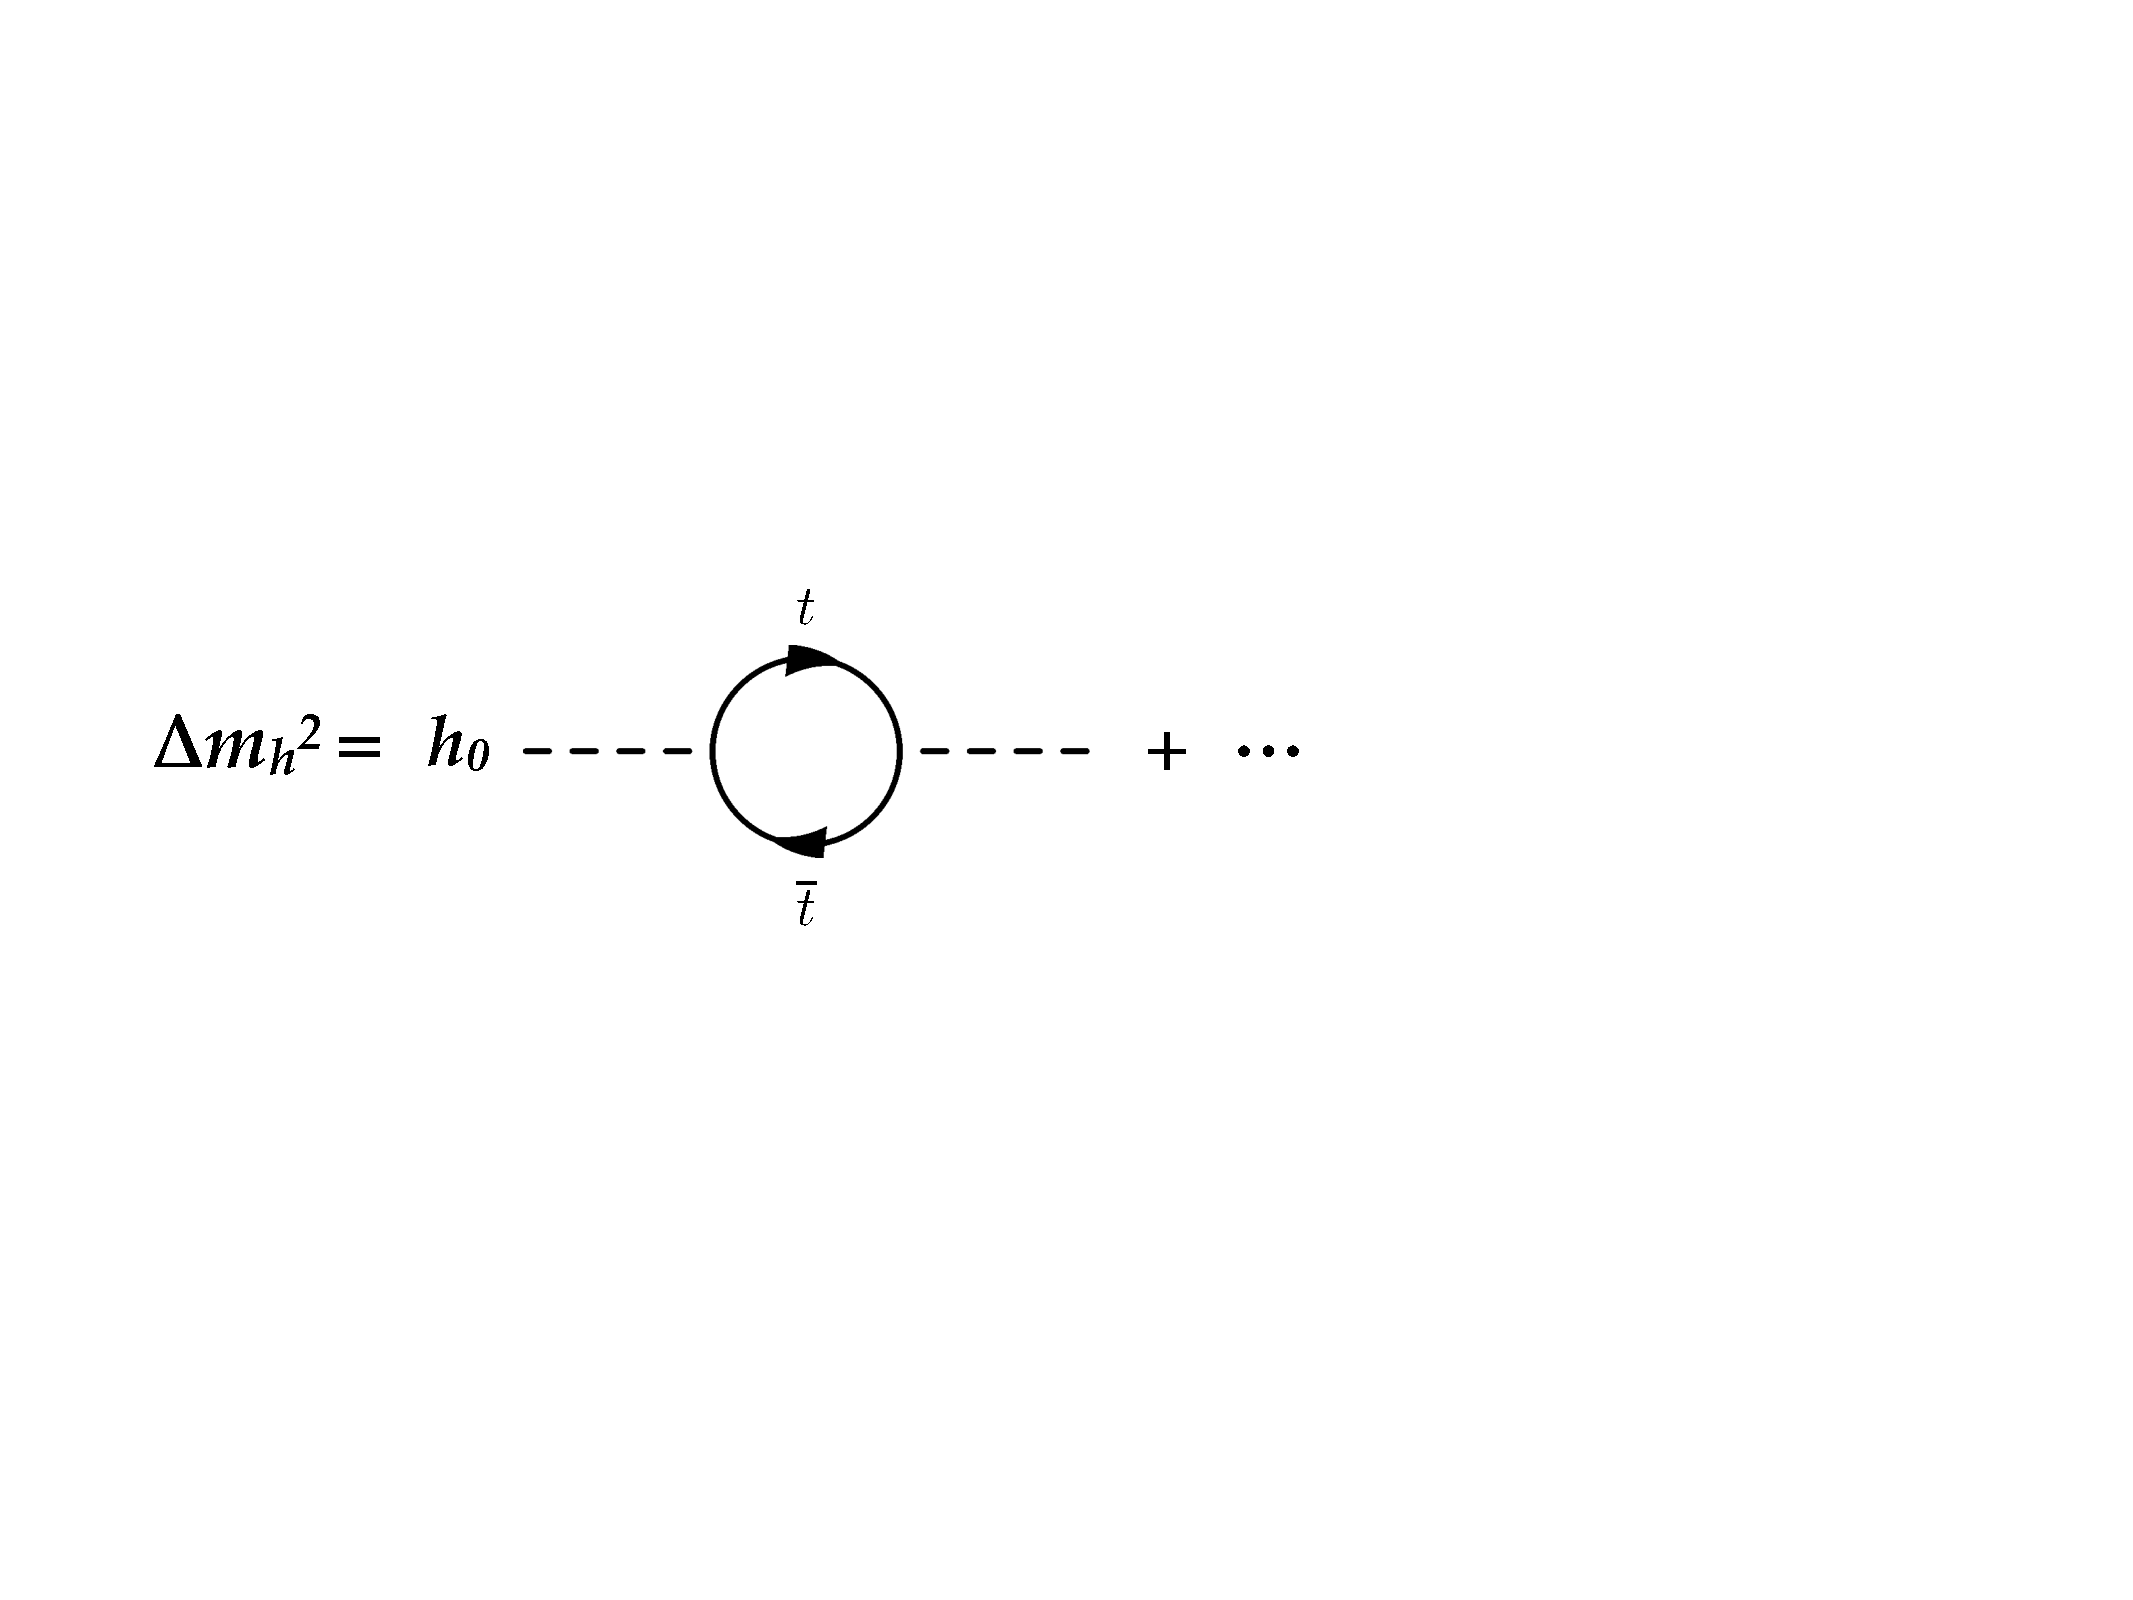
\includegraphics[width=0.6\textwidth]{figures/higgs_corr/higgs_mass_correctionsPDF}
                \caption{
                    Top-quark loop contribution to the higher-order computation of the Higgs mass that
                    leads to unregulated divergent terms such as Equation~\ref{eq:higgs_divergence}.
                }
                \label{fig:higgs_mass_correction}
            \end{center}
        \end{minipage}
        \end{figure}
        The apparent contradiction that the electroweak scale at which the Higgs boson is experimentally known to exist
        should also be unavoidably sensitive to $M_P$, attempting to drive the Higgs boson mass to values 16 orders
        of magnitude larger than the measured one,
        is at the heart of the Hierarchy Problem.
        The high energy scales at which SM calculations fail are typically assumed to be the scales
        at which new physics arise and take over as a more complete description of natural phenomena.
        That the Higgs boson is apparently driven to these scales motivates the arguments in favor
        of their being new physics at or near the electroweak scale which act to cancel the quadratically
        divergent terms appearing in the Higgs mass corrections.
        That cancellations of terms on the order of $10^{30}$ ($\Lambda^2$) should be possible introduces the
        philosophical concerns of \textit{naturalness}, which ponder whether or not Nature is such
        that the additional sources of high energy physics --- not accounted for by the SM --- can conspire in such a way as to
        allow for such perfectly fine-tuned cancellation.
\end{description}



%\section{Particles and Forces}
%
%Here we introduce the SM particle content and provide a description of the interactions that
%link the particles together.
%
%
\begin{table}[!htb]
    \caption{
        The particle content of the SM and their transformation
        properties under the SM gauge groups, prior to electroweak symmetry breaking.
        The representations of each of the gauge groups are shown in the three-right
        columns. The \Uone symmetry of weak-hypercharge transformations is one-dimensional
        and the column gives the weak-hypercharge $\mathcal{Y}$ associated with each
        field. For \SUthree and \SUtwo, $\mathbf{1}$ refers to the field belonging to
        the associated singlet representation, $\mathbf{2}$ to the doublet representation,
        $\mathbf{3}$ to the triplet representation, and $\mathbf{8}$ to the octet representation.
    }
    \begin{center}
        \begin{tabularx}{0.96\textwidth}{m{1em} c c c c c c c }
        \toprule
        \hline
        & Field Label & Content & Spin & \Uone~($\mathcal{=Y}$) & \SUtwo & \SUthree \\
        \hline
        \rotatebox{90}{\hspace{-0.1cm}\textbf{Quarks} } 
         &   \makecell{\fieldQi \\ \fieldUri \\ \fieldDri} % FIELD
         &   \makecell{ (\fieldUl, \fieldDl), (\fieldCl, \fieldSl), (\fieldTl, \fieldBl) \\ \fieldUr \\ \fieldDr}% CONTENT
         &   \makecell{ $1/2$ \\ $1/2$ \\ $1/2$} % SPIN
         &   \makecell{ $1/3$ \\ $4/3$ \\ $-2/3$}% U(1)
         &   \makecell{ $\mathbf{2}$ \\ $\mathbf{1}$ \\ $\mathbf{1}$}% SU(2)
         &   \makecell{ $\mathbf{3}$ \\ $\mathbf{3}$ \\ $\mathbf{3}$}\\ % SU(3)
        %\cdashline{1-7}
        \rotatebox{90}{\hspace{-0.1cm}\textbf{Leptons} }
         &   \makecell{\fieldLi \\ \fieldEri} % FIELD
         &   \makecell{ (\fieldEl, \fieldNuEl), (\fieldMul, \fieldNuMul), (\fieldTaul, \fieldNuTaul) \\ \fieldEr, \fieldMur, \fieldTaur}% CONTENT
         &   \makecell{ $1/2$ \\ $1/2$ }% SPIN
         &   \makecell{ $-1$ \\ $-2$ }% U(1)
         &   \makecell{ $\mathbf{2}$ \\ $\mathbf{1}$ }% SU(2)
         &   \makecell{ $\mathbf{1}$ \\ $\mathbf{1}$ } \\ % SU(3)
        \midrule
        \rotatebox{90}{\textbf{\stackanchor{Gauge}{Fields}} }
         &   \makecell{\fieldB \\ \fieldW \\ \fieldG } % FIELD
         &   \makecell{ \fieldB \\ (\fieldWone, \fieldWtwo, \fieldWthree) \\ \fieldG$_a$, $a\in[1,..,8]$ }% CONTENT
         &   \makecell{ $1$ \\ $1$ \\ $1$} % SPIN
         &   \makecell{ $0$ \\ $0$ \\ $0$}% U(1)
         &   \makecell{ $\mathbf{1}$ \\ $\mathbf{3}$ \\ $\mathbf{1}$}% SU(2)
         &   \makecell{ $\mathbf{1}$ \\ $\mathbf{1}$ \\ $\mathbf{8}$}\\ % SU(3)
        \midrule
        \rotatebox{90}{\textbf{\stackanchor{Higgs}{Field}}} 
         &   \makecell{\fieldPhi } % FIELD
         &   \makecell{ (\fieldPhip, \fieldPhizero) }% CONTENT
         &   \makecell{ $0$  } % SPIN
         &   \makecell{ $1$  }% U(1)
         &   \makecell{ $\mathbf{2}$ }% SU(2)
         &   \makecell{ $\mathbf{1}$ }\\ % SU(3)
        \hline
        \bottomrule
        \end{tabularx}
    \end{center}
    \label{tab:sm_content}
\end{table}
\FloatBarrier

%
\begin{table}[!htb]
    \caption{
        The table shows the particle fields of the SM after SSB. Coupling and mass parameters are provided. 
    }
        %The particle content of the SM after the process of
        %electroweak symmetry breaking.
        %Shown for each particle species are the associated electric charge, $Q$,
        %coupling, and mass (approximate).
        %The $y_i$ are the Yukawa coupling (Equation~\ref{eq:higgs_fermion_coupling}),
        %$\alpha_{\text{EM}}$ is the QED coupling constant (`fine structure constant'),
        %$\mathcal{V}$ indicates the parameters of the CKM matrix, and
        %$\alpha_s$ is the QCD coupling constant.
        %The quantities $\lambda$ and $\mu$ are the Higgs self-coupling parameter
        %and mass terms, respectively, appearing in Higgs potential terms (Equation~\ref{eq:higgs_potential}).
    \begin{center}
        \begin{tabularx}{1\textwidth}{m{1em} c c c c }
        \toprule
        \hline
        & Physical Field & Q & Coupling & Mass [GeV] \\
        \hline
        \rotatebox{90}{\hspace{-0.1cm}\textbf{Quarks} } 
            & \makecell{ \quarkU, \quarkC, \quarkT \\ \quarkD, \quarkS, \quarkB} % FIELD
            & \makecell{ $2/3$ \\ $-1/3$ }% Q
            %& \makecell{ $\mathbf{3}$ \\ $\mathbf{3}$ } % SU(3)
            & \makecell{ ($y_i=$) $1\times10^{-5}$, $7\times10^{-3}$, $1$ \\ ($y_i=$) $3\times10^{-5}$, $5\times10^{-4}$, $0.02$ } % Coupling
            & \makecell{ $2\times10^{-3}$, $1.27$, $173$ \\ $4\times10^{-4}$, $0.10$, $4.18$ }\\% Mass
        \rotatebox{90}{\hspace{-0.1cm}\textbf{Leptons} } 
            & \makecell{ \leptonE, \leptonMu, \leptonTau \\ \neutrinoE, \neutrinoMu, \neutrinoTau } % FIELD
            & \makecell{ $-1$ \\ $0$ }% Q
            %& \makecell{ $\mathbf{1}$ \\ $\mathbf{1}$ } % SU(3)
            & \makecell{ ($y_i=$) $3\times10^{-7}$, $6\times10^{-4}$, $0.01$ \\ -- } % Coupling
            & \makecell{ $5\times10^{-4}$, $0.106$, $1.777$ \\ --}\\% Mass
        \midrule
        \rotatebox{90}{\textbf{Bosons} } 
            & \makecell{ \fieldPhoton \\ \fieldZ \\ (\fieldWp, \fieldWm) \\ \fieldG } % FIELD
            & \makecell{ $0$ \\ $0$ \\ $(+1,-1)$ \\ $0$ }% Q
            %& \makecell{ $\mathbf{1}$ \\ $\mathbf{1}$ \\ $\mathbf{1}$ \\ $\mathbf{8}$ } % SU(3)
            & \makecell{ $\alpha_{\text{EM}} \simeq 1/137$ \\ $\sin \theta_{W} \simeq 0.5$ \\ $\mathcal{V}_{\text{CKM}}$ \\ $\alpha_s \simeq 0.1$ } % Coupling
            & \makecell{ $0$ \\ $91.2$ \\ $80.4$ \\  $0$}\\% Mass
        \midrule
        \rotatebox{90}{\textbf{Higgs} } 
            & \makecell{ \fieldH } % FIELD
            & \makecell{ $0$ }% Q
            %& \makecell{ $\mathbf{1}$ } % SU(3)
            & \makecell{ $\lambda$, $\mu$ } % Coupling
            & \makecell{ $125.09$ }\\% Mass
        \hline
        \bottomrule
        \end{tabularx}
    \end{center}
    \label{tab:sm_content_EWSB}
\end{table}



%\subsection{Gauge Theories}

%\subsubsection{The Electroweak Theory}


